\documentclass[letterpaper,twoside]{article}
\usepackage{aistats2027}
\usepackage{amssymb,amsthm,mathtools,bm,microtype,enumitem,graphicx,booktabs}
\usepackage[colorlinks=true,linkcolor=blue,citecolor=blue,urlcolor=blue]{hyperref}
\usepackage[nameinlink,capitalize,noabbrev]{cleveref}
\newtheorem{theorem}{Theorem}[section]
\newtheorem{proposition}[theorem]{Proposition}
\newtheorem{lemma}[theorem]{Lemma}
\newtheorem{corollary}[theorem]{Corollary}
\theoremstyle{definition}
\newtheorem{definition}[theorem]{Definition}
\theoremstyle{remark}
\newtheorem{remark}[theorem]{Remark}

\newcommand{\R}{\mathbb R}
\newcommand{\N}{\mathbb N}
\newcommand{\cP}{\mathcal P}
\newcommand{\cM}{\mathcal M}
\newcommand{\supp}{\operatorname{supp}}
\newcommand{\spec}{\operatorname{spec}}
\newcommand{\diag}{\operatorname{diag}}
\newcommand{\Var}{\operatorname{Var}}
\newcommand{\ip}[2]{\langle #1,#2\rangle}
\newcommand{\norm}[1]{\lVert #1\rVert}
\newcommand{\doi}[1]{\href{https://doi.org/#1}{doi:#1}}


\renewcommand{\thesection}{S\arabic{section}}
\hypersetup{pdftitle={Periodic Barzilai--Borwein Switching: Supplementary Material},pdfauthor={}}
\makeatletter
\renewcommand{\Notice@String}{Research working paper. Author review pending.}
\makeatother
\begin{document}
\onecolumn
\aistatstitle{Periodic Barzilai--Borwein Switching:\\Supplementary Material}
\fancyhead[CE,CO]{\small\bfseries Research working paper}
\noindent\textbf{Research working paper.} AI-assisted preparation. Author review pending. This supplement gives the complete theoretical development, including all assumptions, proofs, initialization conventions, and additional cycle classification. The main manuscript presents the central phase-balance and strict-gap results. Section and theorem numbers here are local to the supplement.

The fixed-selector spectral-measure and endpoint-band method is due to Yang and Yuan~\cite{YangYuan2026}. The later endpoint Lyapunov and closed-cone envelope formulations are also established \cite{YangYuanLyapunov2026,YangYuanCone2026}. Stepwise alternation is an existing algorithm~\cite{GrippoSciandrone2002,DaiFletcherProjected2005}. The three-point reciprocal pair and its per-step factor have the algebraic antecedent in cyclic BB~\cite{DaiHagerSchittkowskiZhang2006}. The present claims concern periodic phase compatibility, the sharp envelope threshold, quantitative gaps, and the exact unrestricted cubic coefficient near isotropy. Section~\ref{sec:exact-local} strengthens the earlier cubic-order bounds retained below.

\section{Periodic delayed spectral selectors}\label{sec:setting}

Let $\mathcal H$ be a real Hilbert space and let
\begin{equation}\label{eq:operator-bounds}
 A=A^*\in\mathcal L(\mathcal H),
 \qquad 0<aI\le A\le bI<\infty,
 \qquad a<b.
\end{equation}
For
\[
 q(x)=\frac12\ip{Ax}{x}-\ip{d}{x},
\]
the minimizer is $x_*=A^{-1}d$ and
$g_k=A(x_k-x_*)$.  We allow an arbitrary positive warm-up step
$\alpha_0>0$.  The first prescribed phase is phase zero and is applied to
the transition $g_1\mapsto g_2$.

Write $K=[a,b]$ and let $\cP(K)$ be the Borel probability measures on $K$,
equipped with the topology of weak convergence (equivalently, the weak-star
topology inherited from $C(K)^*$).
A \emph{delayed spectral selector} is a continuous map
\[
 U:\cP(K)\to K
\]
with the internality property
\begin{equation}\label{eq:internality}
 \min\supp\nu\le U(\nu)\le\max\supp\nu
 \qquad(\nu\in\cP(K)).
\end{equation}
For a period $L\ge1$, fix
$\bm U=(U_0,\ldots,U_{L-1})$ and set
\begin{equation}\label{eq:selector-iteration}
 \alpha_k=\frac1{U_j(\nu_{k-1})},
 \qquad g_{k+1}=\left(I-\frac{A}{U_j(\nu_{k-1})}\right)g_k,
  \qquad j=k-1\pmod L,\qquad k\ge1,
\end{equation}
where $\nu_k$ is the normalized scalar spectral measure of $g_k$:
\begin{equation}\label{eq:scalar-measure}
 \nu_k(B)=\frac{\ip{E_A(B)g_k}{g_k}}{\norm{g_k}^2}.
\end{equation}
Finite termination is followed by zero extension.
With the phase convention in \eqref{eq:selector-iteration}, the warm-up is
called \emph{phase-zero matched} if
\begin{equation}\label{eq:general-matched-warmup}
 \alpha_0=\frac1{U_0(\nu_0)}.
\end{equation}
Thus the warm-up and the first prescribed quotient use the same gradient and
the same phase selector.  The phase-$j$ definition is obtained by cyclically
rotating the selector schedule.

Two classes will be used repeatedly.  A positive spectral weight
$\Psi_j\in C(K;(0,\infty))$ gives
\begin{equation}\label{eq:weighted-selector}
 U_j(\nu)=
 \frac{\int_K\lambda\Psi_j(\lambda)\,d\nu(\lambda)}
      {\int_K\Psi_j(\lambda)\,d\nu(\lambda)}.
\end{equation}
The choices $\Psi\equiv1$ and $\Psi(\lambda)=\lambda$ are BB1 and BB2.
The convex BB family of \cite{DaiHuangLiu2019} gives instead
\begin{equation}\label{eq:convex-selector}
 \frac1{U_\gamma(\nu)}
 =\gamma\frac1{\int\lambda\,d\nu}
 +(1-\gamma)\frac{\int\lambda\,d\nu}{\int\lambda^2\,d\nu}.
\end{equation}
Both constructions are continuous and satisfy \eqref{eq:internality}.

If the warm-up itself gives $g_1=0$, we set all three root factors below to
zero.  For every remaining nonterminal trajectory, define the gradient,
error, and objective-gap root factors by
\begin{align}
 \rho_g&=\limsup_{k\to\infty}
 \left(\frac{\norm{g_k}}{\norm{g_1}}\right)^{1/k},
 &
 \rho_x&=\limsup_{k\to\infty}
 \left(\frac{\norm{x_k-x_*}}{\norm{x_1-x_*}}\right)^{1/k},
 \label{eq:root-factors}
 \rho_q&=\limsup_{k\to\infty}
 \left(\frac{q(x_k)-q(x_*)}{q(x_1)-q(x_*)}\right)^{1/k}.
\end{align}
Under zero extension, a finitely terminating trajectory has all three root
factors equal to zero.
Deleting a finite prefix leaves the root factor unchanged.  For fixed $g_0$,
the warm-up may nevertheless change the post-warm-up projective state and the
attained factor.  Uniform estimates over all $\alpha_0>0$ are therefore
normalized by $\norm{g_1}$; normalization by $\norm{g_0}$ admits no
warm-up-independent constant.

\subsection{The phase-lifted normalized dynamics}

For $u\in K$ and $w\in\cP(K)$ set
\begin{equation}\label{eq:replicator}
 Q_u(\lambda)=\left(1-\frac\lambda u\right)^2,
 \qquad
 R_u(w)=\int_K Q_u(\lambda)\,dw(\lambda)
\end{equation}
and, whenever $R_u(w)>0$, define the probability $F_u w$ setwise by
\begin{equation}\label{eq:replicator-measure}
 (F_u w)(B)=
 \frac{\int_B Q_u(\lambda)\,dw(\lambda)}{R_u(w)}
 \qquad\text{for every Borel }B\subset K.
\end{equation}
The square root of $R_u(w)$ is the one-step gradient
norm ratio.  On
\[
 X_0=\cP(K)^2\times\mathbb Z_L,
 \qquad \mathbb Z_L=\mathbb Z/L\mathbb Z,
\]
define, at regular states,
\begin{equation}\label{eq:phase-map}
 T(w,z,j)=\bigl(F_{U_j(z)}w,w,j+1\!\!\pmod L\bigr),
 \qquad
 f(w,z,j)=\frac12\log R_{U_j(z)}(w).
\end{equation}
Adjoin an isolated terminal point $\theta$ and put
\[
 D=\{\theta\}\cup
 \{(w,z,j)\in X_0:R_{U_j(z)}(w)=0\}.
\]
Every point of $D$ is sent to $\theta$, and $f=-\infty$ on $D$.  The
resulting space $X=X_0\sqcup\{\theta\}$ is compact and metrizable.  The map
$T$ is Borel and continuous on $X\setminus D$; $f$ is upper semicontinuous
and bounded above.

For a probability measure $\mu$ on $X$, define the extended integral by
\[
 f_M=\max\{f,-M\},
 \qquad
 \int f\,d\mu=\lim_{M\to\infty}\int f_M\,d\mu.
\]
Since $f$ is bounded above, this limit belongs to $[-\infty,\infty)$.  If
$\int f\,d\mu> -\infty$, then $\mu(D)=0$ and $f\in L^1(\mu)$.

The cocycle identity is
\begin{equation}\label{eq:cocycle}
 \log\frac{\norm{g_{n+1}}}{\norm{g_1}}
 =\sum_{k=1}^{n}f(T^{k-1}\chi_1),
 \qquad \chi_1=(\nu_1,\nu_0,0).
\end{equation}

\section{Invariant averages and the strict-gap principle}\label{sec:invariant}

\subsection{Persistent supports and endpoint rigidity}

Set
\begin{equation}\label{eq:cab}
 c(a,b)=\frac{b-a}{b+a},
 \qquad m(a,b)=\frac{a+b}{2}.
\end{equation}
The elementary endpoint inequality
\begin{equation}\label{eq:endpoint-inequality}
 \left(\frac{u-a}{u}\right)^{b/(a+b)}
 \left(\frac{b-u}{u}\right)^{a/(a+b)}
 \le c(a,b)
\end{equation}
holds for $u\in[a,b]$, with equality only at $u=m(a,b)$.

The following selector-independent lemma captures the equality mechanism.

\begin{lemma}[persistent support]\label{lem:persistent-support}
Let $\Pi$ be an ergodic $T$-invariant probability measure with
$\int f\,d\Pi> -\infty$.  There is a compact set $S\subset K$ containing at
least two points such that
\[
 \supp w=\supp z=S
 \qquad\text{for $\Pi$-almost every }(w,z,j).
\]
Moreover, the phase marginal of $\Pi$ is uniform on $\mathbb Z_L$.
\end{lemma}

\begin{proof}
Finite average gives $\Pi(D)=0$.  Let $\mathcal U$ be a countable base of the
relative topology of $K$ and put
\[
 b_V(w,z,j)=\mathbf1_{\{w(V)>0\}},
 \qquad b_V(\theta)=0
 \qquad(V\in\mathcal U).
\]
Absolute continuity
$F_u w\ll w$ gives $b_V\circ T\le b_V$.  Invariance makes the integrals equal,
so $b_V\circ T=b_V$ almost surely; ergodicity makes $b_V$ almost surely zero
or one.  Define the first-coordinate barycenter by
\[
 \bar w(B)=\int_X w(B)\,d\Pi(w,z,j)
\]
and set $S=\supp\bar w$.  For every $V\in\mathcal U$,
\[
 \bar w(V)>0
 \quad\Longleftrightarrow\quad
 \Pi\{w(V)>0\}>0
 \quad\Longleftrightarrow\quad
 w(V)>0\quad\Pi\text{-almost surely}.
\]
Intersecting these events over the countable base and using the neighborhood
characterization of support gives $\supp w=S$ almost surely.  On the regular
set, the second coordinate of $T(w,z,j)$ is $w$; invariance therefore makes
the first and second coordinate marginals equal and gives $\supp z=S$ almost
surely.  A further countable intersection gives the same statement along all
forward iterates.  If $S$ were a singleton, internality would make the next
multiplier vanish on the whole support, placing the state in $D$, a
contradiction.
Set
\[
 r_j=\Pi\bigl(\cP(K)^2\times\{j\}\bigr),
 \qquad j\in\mathbb Z_L.
\]
Since the phase advances by one almost surely, invariance gives
$r_{j+1}=r_j$ for every $j$, and hence $r_j=1/L$.
\end{proof}

\begin{lemma}[endpoint-band bound and rigidity]\label{lem:endpoint-band}
Let $\Pi$ be as in \cref{lem:persistent-support}, and let
$a_S=\min S$, $b_S=\max S$.  Then
\begin{equation}\label{eq:invariant-bound}
 \int f\,d\Pi\le\log c(a_S,b_S)\le\log c(a,b).
\end{equation}
If equality holds with the rightmost quantity, then $a_S=a$, $b_S=b$, and
\begin{equation}\label{eq:equality-rigidity}
 U_j(z)=m(a,b),
 \qquad
 w\bigl(K\setminus\{a,b\}\bigr)
 =z\bigl(K\setminus\{a,b\}\bigr)=0
\end{equation}
for $\Pi$-almost every state.  Both endpoint masses are then strictly
positive almost surely.
\end{lemma}

\begin{proof}
See \cref{sec:endpoint-band-proof}.
\end{proof}

\begin{remark}
The invariant bound \eqref{eq:invariant-bound} is not a pointwise contraction
estimate; individual norm ratios may exceed $c(a,b)$.
\end{remark}

\subsection{The maximal invariant factor and its realization}

Let $\cM_T(X)$ denote the $T$-invariant Borel probability measures on $X$.
Define the maximal invariant log-growth and its exponential by
\begin{equation}\label{eq:beta-gamma}
 \beta_{\bm U}(a,b)
 =\sup_{\Pi\in\cM_T(X)}\int f\,d\Pi,
 \qquad
 \Gamma_{\bm U}(a,b)=e^{\beta_{\bm U}(a,b)}.
\end{equation}
Here $e^{-\infty}=0$. We do not presuppose $\Gamma_{\bm U}>0$ for arbitrary continuous internal selectors. Periodic positive spectral weights and binary BB words considered below have positive invariant factor.

Let $q^{\rm H}_{\bm U}(a,b)$ be the supremum of $\rho_g$ over all real
Hilbert spaces, all operators satisfying \eqref{eq:operator-bounds}, all
nonzero initial gradients, and all positive warm-up steps, with phase zero
applied first.  Let $q^{\rm fd}_{\bm U}(a,b)$ denote the same supremum
restricted to finite-dimensional spaces.  Thus
$q^{\rm fd}_{\bm U}\le q^{\rm H}_{\bm U}$.

\begin{lemma}[attainment of the maximal average]\label{lem:max-attained}
If $\beta_{\bm U}(a,b)>-\infty$, the supremum in
\eqref{eq:beta-gamma} is attained by an invariant probability measure of
finite $f$-average.  Moreover, an ergodic maximizing invariant probability
may be chosen.
\end{lemma}

\begin{proof}
The potential is bounded above, so $\beta_{\bm U}<\infty$.  Let $\Pi_n$ be an
invariant maximizing sequence with finite averages and, after passing to a
subsequence, suppose $\Pi_n\Rightarrow\Pi$.  For every $M>0$, the lower
truncation $f_M=\max\{f,-M\}$ is bounded and upper semicontinuous.
Portmanteau gives
\[
 \limsup_{n\to\infty}\int f_M\,d\Pi_n
 \le\int f_M\,d\Pi.
\]
Since $f_M\ge f$,
\[
 \beta_{\bm U}\le\int f_M\,d\Pi
 \qquad(M>0).
\]
Letting $M\to\infty$ according to the extended-integral convention yields
$\beta_{\bm U}\le\int f\,d\Pi$, and in particular $\Pi(D)=0$.

Weak limits of invariant measures need not be invariant for a merely Borel
map, so the null-set conclusion is essential.  If $\varphi\in C(X)$, every
discontinuity of the bounded Borel function $\varphi\circ T$ lies in $D$.
The weak-convergence theorem for bounded functions that are continuous
$\Pi$-almost everywhere \cite[Sec.~2]{Billingsley1999} therefore passes the
invariance identities of $\Pi_n$ to $\Pi$.  Hence
$\Pi$ is invariant, and the definition of $\beta_{\bm U}$ gives the reverse
inequality.

Decompose $\Pi$ into ergodic invariant probabilities.  If $C$ is an
upper bound for $f$, apply the decomposition identity and Tonelli's theorem
to $C-f\ge0$.  Almost every component has finite $f$-average, their averages
integrate to $\beta_{\bm U}$, and each is at most $\beta_{\bm U}$.  Thus
almost every component is maximizing, and one may be chosen.
\end{proof}

We prove the following extended-real Borel-map bound in the spirit of the semi-uniform principle \cite{SturmanStark2000}; compare the fixed-rule implementation in \cite{YangYuan2026}.

\begin{proposition}[semi-uniform ergodic bound]\label{prop:semiuniform}
Let $X$ be a compact metric space, let $T:X\to X$ be Borel, and let $D\subset X$ be
a Borel set containing all discontinuities of $T$.  Suppose that
$f:X\to[-\infty,\infty)$ is upper
semicontinuous, bounded above, and equals $-\infty$ on $D$.  If
\[
 \int f\,d\mu\le\beta
\]
for some $\beta\in\R$ and every invariant probability measure of finite
$f$-average, then for every $\eta>0$ there is $B_\eta<\infty$ such that
\[
 \sum_{k=0}^{n-1}f(T^kx)
 \le n(\beta+\eta)+B_\eta
\]
for every orbit segment avoiding $D$.
\end{proposition}

\begin{proof}
Suppose first that no common long-segment bound holds.  Then there are regular
orbit segments $(x_\ell,n_\ell)$ with $n_\ell\to\infty$ such that
\[
 \frac1{n_\ell}\sum_{k=0}^{n_\ell-1}f(T^kx_\ell)
 >\beta+\eta.
\]
Let
\[
 \mu_\ell=\frac1{n_\ell}
 \sum_{k=0}^{n_\ell-1}\delta_{T^kx_\ell}
\]
and, after passing to a subsequence, suppose that $\mu_\ell\Rightarrow\mu$.
For $f_M=\max\{f,-M\}$, Portmanteau gives
\[
 \limsup_{\ell\to\infty}\int f_M\,d\mu_\ell
 \le\int f_M\,d\mu.
\]
Since $f\le f_M$, this implies, for every $M$,
\[
 \limsup_{\ell\to\infty}\int f\,d\mu_\ell
 \le\int f_M\,d\mu.
\]
Letting $M\to\infty$ according to the extended-integral convention yields
\[
 \int f\,d\mu
 \ge\limsup_{\ell\to\infty}\int f\,d\mu_\ell
 \ge\beta+\eta.
\]
The finite lower bound implies $\mu(D)=0$.

For every $\varphi\in C(X)$,
\[
 \int(\varphi\circ T-\varphi)\,d\mu_\ell
 =\frac{\varphi(T^{n_\ell}x_\ell)-\varphi(x_\ell)}{n_\ell}
 \longrightarrow0.
\]
Every discontinuity of the bounded Borel function $\varphi\circ T$ lies in
the $\mu$-null set $D$.  The same weak-convergence theorem for bounded
$\mu$-almost-everywhere continuous functions
\cite[Sec.~2]{Billingsley1999} passes this identity to the limit, proving that
$\mu$ is invariant.  This contradicts the assumed
invariant-average bound.  Thus there is $N$ such that every regular segment
of length $n\ge N$ has average at most $\beta+\eta$.

If $C$ is an upper bound for $f$, the finitely many lengths $1\le n<N$ are
covered by
\[
 B_\eta=(N-1)\max\{0,C-\beta-\eta\}.
\]
This proves the proposition.
\end{proof}

\begin{theorem}[realization of the invariant factor]
\label{thm:gamma-realization}
For every periodic selector family satisfying \eqref{eq:internality},
\begin{equation}\label{eq:gamma-algorithmic}
 q^{\rm H}_{\bm U}(a,b)=\Gamma_{\bm U}(a,b).
\end{equation}
Thus $\Gamma_{\bm U}$ is the exact worst-case trajectory root factor over the
Hilbert problem class.
\end{theorem}

\begin{proof}
Suppose first that $\beta_{\bm U}>-\infty$.  Every invariant probability of
finite $f$-average has average at most $\beta_{\bm U}$.  Applying
\cref{prop:semiuniform} with benchmark $\beta_{\bm U}$ gives, for every
$\eta>0$,
\[
 \limsup_{n\to\infty}\frac1n
 \sum_{t=0}^{n-1}f(T^tx)\le\beta_{\bm U}+\eta
\]
on every regular forward orbit.  The cocycle \eqref{eq:cocycle} and then
$\eta\downarrow0$ give $\rho_g\le e^{\beta_{\bm U}}$.

If $\beta_{\bm U}=-\infty$, there is no invariant probability of finite
$f$-average.  Thus \cref{prop:semiuniform} applies with any finite benchmark
$b_0$.  Taking, for example, $\eta=1$ gives
$\rho_g\le e^{b_0+1}$; letting $b_0\to-\infty$ yields
 $q^{\rm H}_{\bm U}=0=\Gamma_{\bm U}$.  This proves the upper bound in all
cases.

Suppose now that $\beta_{\bm U}>-\infty$.  By
\cref{lem:max-attained}, choose an ergodic maximizing measure.  Its phase
marginal is uniform by \cref{lem:persistent-support}.  Choose a Birkhoff
generic point in phase $L-1$ whose whole forward orbit is regular,
\[
 x=(w,z,L-1).
\]
Put $u=U_{L-1}(z)$ and
\[
 y=Tx=(F_u w,w,0).
\]
The forward $f$-average of $y$ is still $\beta_{\bm U}$.

Realize the compatible pair on the real Hilbert space
$\mathcal H=L^2(K,w;\R)$.  Let $A$ be multiplication by $\lambda$ and take
the quadratic with $d=0$.  Let $g_0(\lambda)=1$, set $x_0=A^{-1}g_0$, and
choose the positive warm-up $\alpha_0=1/u$.  Then
\[
 g_1(\lambda)=1-\frac\lambda u,
 \qquad \nu_1=F_u w,
\]
so the phase-zero lifted state after the warm-up is exactly $y$.  The cocycle
and Birkhoff genericity give
\[
 \lim_{n\to\infty}
 \frac1{n+1}\log\frac{\norm{g_{n+1}}}{\norm{g_1}}
 =\lim_{n\to\infty}\frac{n}{n+1}
   \frac1n\sum_{t=0}^{n-1}f(T^ty)
 =\beta_{\bm U}.
\]
Hence this Hilbert-space quadratic trajectory has gradient root factor
$e^{\beta_{\bm U}}$, proving the reverse inequality in
\eqref{eq:gamma-algorithmic}.
\end{proof}

\subsection{Finite-dimensional uniform-envelope exactness}

The maximizing measure in \eqref{eq:gamma-algorithmic} may have infinite
support.  The next theorem gives the corresponding exact finite-dimensional
uniform-envelope interpretation.

Define the dimension-free finite-dimensional uniform-envelope threshold by
\begin{equation}\label{eq:fd-envelope-threshold}
\begin{split}
 \Theta^{\rm fd}_{\bm U}(a,b)=\inf\{\tau>0:\ &\text{there exists }C_\tau\ge1
 \text{ such that, for every finite-dimensional problem,}\\
 &\text{every }g_0\ne0,\ \alpha_0>0,\text{ and }k\ge1,\quad
 \norm{g_k}\le C_\tau\tau^{k-1}\norm{g_1}\}.
\end{split}
\end{equation}
The quantifier over finite-dimensional problems includes every dimension and
every symmetric $A$ satisfying \eqref{eq:operator-bounds}; phase zero is
applied first, and terminated trajectories are zero-extended.

\begin{theorem}[finite-dimensional uniform-envelope exactness]
\label{thm:fd-envelope-exact}
For every periodic selector family satisfying \eqref{eq:internality},
\begin{equation}\label{eq:fd-envelope-equality}
 \Theta^{\rm fd}_{\bm U}(a,b)=\Gamma_{\bm U}(a,b).
\end{equation}
Consequently
\begin{equation}\label{eq:rate-hierarchy}
 q^{\rm fd}_{\bm U}(a,b)
 \le q^{\rm H}_{\bm U}(a,b)
 =\Theta^{\rm fd}_{\bm U}(a,b)
 =\Gamma_{\bm U}(a,b).
\end{equation}
\end{theorem}

\begin{proof}
If $\tau>\Gamma_{\bm U}$, the semi-uniform argument in the proof of
\cref{thm:gamma-realization} gives
\[
 \norm{g_k}\le C_\tau\tau^{k-1}\norm{g_1}\qquad(k\ge1)
\]
for the entire Hilbert-space class, and hence for its finite-dimensional
subclass.  When $\Gamma_{\bm U}=0$, the same conclusion holds for every
$\tau>0$ by taking an arbitrary finite benchmark below $\log\tau$ in
\cref{prop:semiuniform}.  Thus
$\Theta^{\rm fd}_{\bm U}\le\Gamma_{\bm U}$.

For the reverse inequality suppose $\Gamma_{\bm U}>0$, fix
$0<\tau<\Gamma_{\bm U}$, and let $C\ge1$.  Put
$\beta=\log\Gamma_{\bm U}>\log\tau$.  As in the realization proof, choose a
whole-forward-regular generic state
\[
 y=(F_u w,w,0)
\]
for an ergodic maximizing probability.  If
$S_n(y)=\sum_{t=0}^{n-1}f(T^ty)$, then $S_n(y)/n\to\beta$; hence some $n$
satisfies
\begin{equation}\label{eq:finite-prefix-violation}
 S_n(y)>\log C+n\log\tau.
\end{equation}
Since the first $n$ iterates of $y$ avoid $D$, continuity of $T$ and $f$ off
$D$ shows inductively that the same is true in a neighborhood of $y$ and that
$S_n$ is continuous there.  Finite atomic probabilities are weakly dense in
$\cP(K)$, so choose $w_r\Rightarrow w$ of finite support.  Continuity of $F_u$
at $w$ gives
\[
 y_r=(F_u w_r,w_r,0)\longrightarrow y,
 \qquad S_n(y_r)\longrightarrow S_n(y).
\]
For all sufficiently large $r$, \eqref{eq:finite-prefix-violation} therefore
holds with $y_r$ in place of $y$.

Write $w_r=\sum_{i=1}^{d_r}p_i\delta_{\lambda_i}$ with $p_i>0$.  On
$\R^{d_r}$ take
\[
 A_r=\diag(\lambda_1,\ldots,\lambda_{d_r}),
 \qquad g_0^{(r)}=(\sqrt{p_1},\ldots,\sqrt{p_{d_r}}),
 \qquad \alpha_0=1/u.
\]
Then the post-warm-up lifted state is exactly $y_r$.  The cocycle identity
gives
\[
 \frac{\norm{g_{n+1}^{(r)}}}{\norm{g_1^{(r)}}}
 =e^{S_n(y_r)}>C\tau^n.
\]
Thus no finite constant can give a dimension-free envelope at any
$\tau<\Gamma_{\bm U}$.  This proves the reverse inequality.  If
$\Gamma_{\bm U}=0$, nonnegativity of the infimum and the first paragraph give
equality directly.
\end{proof}

The approximation realizes one finite regular prefix at a time, with a
spectrum whose size may depend on the prefix.  It proves the uniform-envelope
identity but leaves open whether $q^{\rm fd}_{\bm U}=\Gamma_{\bm U}$ and
whether the critical envelope rate is attained.

\subsection{Phase balance and quantitative gaps}

For a phase $j$, define the balanced endpoint set
\begin{equation}\label{eq:balance-set}
 \mathcal B_j(a,b)=
 \left\{p\in(0,1):
 U_j(p\delta_a+(1-p)\delta_b)=m(a,b)\right\}.
\end{equation}

\begin{theorem}[sharp phase-balance criterion]\label{thm:strict-gap}
For every periodic selector family satisfying \eqref{eq:internality},
\begin{equation}\label{eq:strict-gap}
 0\le\Gamma_{\bm U}(a,b)\le c(a,b),
\end{equation}
and
\begin{equation}\label{eq:balance-iff}
 \Gamma_{\bm U}(a,b)=c(a,b)
 \quad\Longleftrightarrow\quad
 \bigcap_{j=0}^{L-1}\mathcal B_j(a,b)\ne\varnothing.
\end{equation}
When the intersection is nonempty, the equality factor is attained on a
two-dimensional endpoint orbit with the matched warm-up
$\alpha_0=1/m(a,b)=2/(a+b)$.  When
\begin{equation}\label{eq:balance-incompatible}
 \bigcap_{j=0}^{L-1}\mathcal B_j(a,b)=\varnothing,
\end{equation}
the second inequality in \eqref{eq:strict-gap} is strict.

For every $\tau\in(\Gamma_{\bm U}(a,b),1)$ there is
$C_\tau<\infty$, depending only on $(a,b,\bm U,\tau)$ and not on the
Hilbert space, operator, initial gradient, or positive warm-up, such that
every nonterminal trajectory satisfies
\begin{equation}\label{eq:tail-envelope}
 \norm{g_k}\le C_\tau\tau^{k-1}\norm{g_1},
 \qquad k\ge1.
\end{equation}
Consequently every trajectory generated from any positive warm-up has
gradient and error root factors at most $\Gamma_{\bm U}(a,b)$ and
objective-gap root factor at most $\Gamma_{\bm U}(a,b)^2$.
\end{theorem}

\begin{proof}
Let $\mu$ be an invariant probability.  If $\int f\,d\mu=-\infty$, the
desired upper bound is immediate.  Otherwise, apply ergodic decomposition to
$C-f\ge0$, where $C$ is an upper bound for $f$.  Almost every component has
finite $f$-average, and \cref{lem:endpoint-band} applies to it.  Integrating
the component bounds gives
\[
 \int f\,d\mu\le\log c(a,b).
\]
Consequently $\beta_{\bm U}\le\log c(a,b)$ and
$\Gamma_{\bm U}\le c(a,b)$.

 Suppose equality holds.  Then $\beta_{\bm U}=\log c(a,b)>-\infty$, so
\cref{lem:max-attained} supplies an ergodic maximizing probability $\Pi$.
The rigidity part of \cref{lem:endpoint-band} gives, almost surely,
\[
 w=p(w)\delta_a+(1-p(w))\delta_b,
 \qquad
 z=p(z)\delta_a+(1-p(z))\delta_b,
 \qquad
 U_j(z)=m(a,b),
\]
with both endpoint masses positive.  At $m=m(a,b)$, the endpoint squared
multipliers equal $c(a,b)^2$, so $F_m w=w$.  Hence
\[
 T(w,z,j)=(w,w,j+1)
\]
on this full-measure set.  Invariance makes $\Pi$ supported on the diagonal
$\{w=z\}$.  There the Borel endpoint-mass function $p(w)=w(\{a\})$ is
invariant, so ergodicity makes it a constant $p_0\in(0,1)$ almost surely.
The phase marginal is uniform by \cref{lem:persistent-support}; therefore
\[
 U_j\bigl(p_0\delta_a+(1-p_0)\delta_b\bigr)=m(a,b)
 \qquad(j\in\mathbb Z_L).
\]
 Thus equality implies that the intersection in \eqref{eq:balance-iff} is
nonempty.

Conversely, choose $p_0$ in that intersection and put
$w_0=p_0\delta_a+(1-p_0)\delta_b$.  Each phase has
$U_j(w_0)=m(a,b)$, while the two endpoint squared multipliers at $m(a,b)$
are equal.  Hence $F_mw_0=w_0$, and the phase-uniform probability on
\[
 \{(w_0,w_0,j):j\in\mathbb Z_L\}
\]
is invariant with $f=\log c(a,b)$.  Therefore
$\Gamma_{\bm U}\ge c(a,b)$, and \eqref{eq:strict-gap} gives equality.
This orbit is realized in $\R^2$ by
$A=\diag(a,b)$, a gradient with normalized squared components
$(p_0,1-p_0)$, and the matched warm-up $\alpha_0=1/m(a,b)$.  This proves
\eqref{eq:balance-iff}; in particular, \eqref{eq:balance-incompatible}
implies the strict gap.

For the envelope, choose a finite $b_0$ with
$\beta_{\bm U}<b_0<\log\tau$ when $\beta_{\bm U}>-\infty$; if
$\beta_{\bm U}=-\infty$, choose any $b_0<\log\tau$.  Every invariant
probability of finite $f$-average has average at most $b_0$.  Apply
\cref{prop:semiuniform} with benchmark $b_0$ and
$\eta=\log\tau-b_0$.  It gives
\[
 \sum_{t=0}^{n-1}f(T^tx)
 \le n\log\tau+B_\eta.
\]
Increasing the constant to cover $k=1$ and using \eqref{eq:cocycle} gives
\eqref{eq:tail-envelope}.  Norm equivalence under
\eqref{eq:operator-bounds} gives the error root factor, and
\[
 \frac1{2b}\norm{g_k}^2
 \le q(x_k)-q(x_*)
 \le\frac1{2a}\norm{g_k}^2
\]
gives the objective-gap root factor $\tau^2$.
Letting $\tau\downarrow\Gamma_{\bm U}(a,b)$ proves the asserted gradient,
error, and objective-gap root-factor bounds.
\end{proof}

\begin{corollary}[periodic spectral weights]\label{cor:weighted-gap}
For the selectors \eqref{eq:weighted-selector}, if two phases satisfy
\[
 \frac{\Psi_i(b)}{\Psi_i(a)}
 \ne\frac{\Psi_j(b)}{\Psi_j(a)},
\]
then
\[
 0<\Gamma_{\bm U}(a,b)<c(a,b),
\]
and \eqref{eq:tail-envelope} holds.
\end{corollary}

\begin{proof}
For $w=p\delta_a+(1-p)\delta_b$, the condition $U_j(w)=m$ is equivalent to
\[
 \Psi_j(a)p=\Psi_j(b)(1-p),
 \qquad
 p=\frac{\Psi_j(b)}{\Psi_j(a)+\Psi_j(b)}.
\]
Distinct endpoint ratios therefore give disjoint singleton balance sets.
It remains to prove positivity.  Put $q_j=\Psi_j(b)/\Psi_j(a)>0$.  On the
endpoint spectrum write
\[
 \nu_k=p_k\delta_a+(1-p_k)\delta_b,
 \qquad
 y_k=\log\frac{p_k}{1-p_k}.
\]
If phase $j=k-1\pmod L$ is used in the transition
$\nu_k\mapsto\nu_{k+1}$, direct calculation gives
\[
 y_{k+1}=y_k-2y_{k-1}+2\log q_j,
 \qquad j=k-1\pmod L.
\]
The homogeneous state matrix has both eigenvalues of modulus $\sqrt2$, so
$1$ is not an eigenvalue of its $L$th power.  The forced recurrence therefore
has a unique real $L$-periodic solution.  Exponentiating gives a full-support
nonterminal endpoint orbit with finite log-growth, and hence
$\Gamma_{\bm U}>0$.
\end{proof}

For binary BB words the compactness gap can be made explicit.  Write
\[
 U^{\rm BB1}(\nu)=\int\lambda\,d\nu,
 \qquad
 U^{\rm BB2}(\nu)=
 \frac{\int\lambda^2\,d\nu}{\int\lambda\,d\nu}.
\]
For $\bm\sigma\in\{0,1\}^L$, let $U_j^{\bm\sigma}$ be $U^{\rm BB1}$
when $\sigma_j=0$ and $U^{\rm BB2}$ when $\sigma_j=1$.  For
$\bm U^{\bm\sigma}=(U_0^{\bm\sigma},\ldots,U_{L-1}^{\bm\sigma})$, abbreviate
\[
 \beta_{\bm\sigma}:=\beta_{\bm U^{\bm\sigma}},\qquad
 \Gamma_{\bm\sigma}:=\Gamma_{\bm U^{\bm\sigma}},\qquad
 q^{\rm H}_{\bm\sigma}:=q^{\rm H}_{\bm U^{\bm\sigma}}.
\]
The following constants give a closed-form, dimension-free certificate for
arbitrary discrete or continuous spectra.

\begin{theorem}[explicit gap for a mixed periodic BB word]
\label{thm:explicit-mixed-gap}
Put
\[
 C=\frac{b-a}{b+a},\qquad
 k_0=\frac{(1-C)^2}{2},\qquad
 H=\frac{3-C}{2(1-C)},\qquad
 Q_C=4+\frac{C}{1-C},
\]
and let $\bm\sigma\in\{0,1\}^L$ be a cyclic word containing both symbols.
Define
\[
 A_L=\frac{(14+C)\sqrt L+2Q_CLH}{\sqrt{k_0}},
 \qquad B_L=2Q_CL,
\]
\begin{equation}\label{eq:explicit-gap-constant}
 \tau_L(C)=
 \frac{2C}{A_L+\sqrt{A_L^2+4C(B_L+C)}},
 \qquad \delta_L(C)=\tau_L(C)^2.
\end{equation}
Then
\begin{equation}\label{eq:explicit-mixed-gap}
 \beta_{\bm\sigma}(a,b)
 \le\log C-\delta_L(C),
 \qquad
 \Gamma_{\bm\sigma}(a,b)
 \le Ce^{-\delta_L(C)}<C.
\end{equation}
\end{theorem}

\begin{remark}[scale of the explicit certificate]
The certificate in \eqref{eq:explicit-mixed-gap} has the following limiting
regimes.  For fixed $L$,
\[
 \delta_L(C)\sim\frac{C^2}{2(14\sqrt L+12L)^2}\quad(C\downarrow0),
 \qquad
 \delta_L(C)\sim\frac{(1-C)^6}{8L^2}\quad(C\uparrow1).
\]
Since $1-C=2/(\kappa+1)$, the second relation is
$\delta_L(C)\sim8/(L^2\kappa^6)$.  For fixed $0<C<1$,
\[
 L^2\delta_L(C)\longrightarrow
 \frac{C^2(1-C)^6}{2(4-3C)^2(3-C)^2}.
\]
Thus the certificate quantifies strict separation uniformly in the dimension,
although it may be conservative for large $\kappa$.
\end{remark}

The proof, given in \cref{sec:quantitative-gap-proof}, combines the endpoint
logarithmic defect with a second defect measuring spectral mass away from the
two persistent endpoints.  At a cyclic $1\to0$ phase boundary, the two
defects prevent a near-extremal orbit from moving its spectral mean far
enough to satisfy both the BB2 and BB1 balance requirements.

\section{Fixed and periodic convex combinations of the BB rules}\label{sec:convex}

We now apply \cref{thm:strict-gap} to the family
\eqref{eq:convex-selector}.  For an endpoint mixture
$w_p=p\delta_a+(1-p)\delta_b$, write
\[
 \alpha^{\rm BB1}(p)=\frac1{ap+b(1-p)},
 \qquad
 \alpha^{\rm BB2}(p)=\frac{ap+b(1-p)}{a^2p+b^2(1-p)},
\]
and
\[
 \alpha_\gamma(p)=\gamma\alpha^{\rm BB1}(p)
 +(1-\gamma)\alpha^{\rm BB2}(p).
\]

\begin{proposition}[fixed mixtures attain the fixed-rule factor]\label{prop:fixed-mixture}
For every $\gamma\in[0,1]$, there is a unique
$p_\gamma\in(0,1)$ such that
\begin{equation}\label{eq:fixed-balance}
 \alpha_\gamma(p_\gamma)=\frac2{a+b}.
\end{equation}
Taking $\nu_0=w_{p_\gamma}$ and the matched warm-up
$\alpha_0=\alpha_\gamma(p_\gamma)=2/(a+b)$ produces an endpoint orbit
with gradient and error root factors $c(a,b)$ and objective-gap root factor
$c(a,b)^2$.  Consequently every fixed convex mixture has sharp worst-case
trajectory root factor
$c(a,b)$.
\end{proposition}

\begin{proof}
Both $\alpha^{\rm BB1}(p)$ and $\alpha^{\rm BB2}(p)$ are strictly increasing
from $1/b$ to $1/a$ as $p$ runs from zero to one.  Hence so is
$\alpha_\gamma$, and
$2/(a+b)$ lies strictly between its endpoint values.  This proves existence
and uniqueness.  At \eqref{eq:fixed-balance}, the two endpoint multipliers
are $c(a,b)$ and $-c(a,b)$, so their squared energies retain the same weights
and the step repeats.  For the upper bound,
\cref{lem:endpoint-band,prop:semiuniform,thm:gamma-realization} give an exact
worst-case trajectory root factor at most $c(a,b)$ for this fixed selector.  The
endpoint orbit attains it.
\end{proof}

The balancing mass moves strictly with the mixing parameter.

\begin{lemma}\label{lem:balance-monotone}
If $0\le\gamma_1<\gamma_2\le1$, then
$p_{\gamma_2}<p_{\gamma_1}$.
\end{lemma}

\begin{proof}
For every $p\in(0,1)$, the moment inequality gives
$\alpha^{\rm BB1}(p)>\alpha^{\rm BB2}(p)$, so $\alpha_\gamma(p)$ is strictly
increasing in $\gamma$.  It is also strictly increasing in $p$.  Maintaining the fixed
value $2/(a+b)$ therefore requires $p$ to decrease when $\gamma$ increases.
\end{proof}

\begin{theorem}[nonconstant periodic mixing yields a strict gap]\label{thm:periodic-mixing}
Let $(\gamma_0,\ldots,\gamma_{L-1})\in[0,1]^L$ be nonconstant and use
$U_j=U_{\gamma_j}$ in \eqref{eq:selector-iteration}.  Abbreviate
$\Gamma_{\bm\gamma}:=\Gamma_{(U_{\gamma_0},\ldots,U_{\gamma_{L-1}})}$.
Then the exact Hilbert worst-case trajectory root factor satisfies
\begin{equation}\label{eq:mixing-gap}
 0\le\Gamma_{\bm\gamma}(a,b)<\frac{b-a}{b+a}
\end{equation}
with all the root-factor and uniform-envelope conclusions of
\cref{thm:strict-gap}.
\end{theorem}

\begin{proof}
By \cref{lem:balance-monotone}, distinct values of $\gamma$ have distinct
singleton balance sets.  Hence \eqref{eq:balance-incompatible} holds, and
\cref{thm:strict-gap} applies.
\end{proof}

Scaling to $a=1$, $b=\kappa$ and writing
$q=p/(1-p)$, the balancing equation is
\begin{equation}\label{eq:qgamma}
 \gamma\frac{q+1}{q+\kappa}
 +(1-\gamma)\frac{q+\kappa}{q+\kappa^2}
 =\frac2{\kappa+1}.
\end{equation}
It has one positive root $q_\gamma$, with
$q_1=1$ and $q_0=\kappa$.  Clearing denominators yields
\[
 q_\gamma^2+\gamma(\kappa^2-1)q_\gamma-\kappa^2=0,
\]
and hence
\begin{equation}\label{eq:qgamma-closed}
 q_\gamma=
 \frac{\sqrt{\gamma^2(\kappa^2-1)^2+4\kappa^2}
       -\gamma(\kappa^2-1)}{2}.
\end{equation}
Implicit differentiation gives $q_\gamma'<0$, which also proves
\cref{lem:balance-monotone}.

For $0<\gamma<1$, the fixed orbit in \cref{prop:fixed-mixture} is not covered
by \cite[Theorem~2]{DaiHuangLiu2019}: its constant endpoint-energy ratio
$q_\gamma\in(1,\kappa)$ makes the quantity in condition~(28) there equal to
$\sqrt2\lvert\log q_\gamma\rvert<8\log\kappa$.

\section{Exact two-point dynamics for a prescribed BB word}\label{sec:two-point}

We specialize to
\[
 A=\diag(1,\kappa),\qquad \kappa>1,
\]
and a prescribed periodic word
$\bm\sigma=(\sigma_0,\ldots,\sigma_{L-1})\in\{0,1\}^L$, where zero denotes
BB1 and one denotes BB2.  To keep the arbitrary warm-up separate from the
prescribed phases, put $h_{-1}=g_0$ and $h_0=g_1$.  For $n\ge0$, the symbol
$\sigma_n$ selects the step formed from $h_{n-1}$ and used in
$h_n\mapsto h_{n+1}$.  The word is extended periodically to all integer
indices only when we describe its periodic response.  Unless stated
otherwise, $L$ is the minimal period.  Cyclic shifts have the same periodic
factor, although the matched-initialization condition is phase dependent.

Write $h_n=(\xi_n,\eta_n)$ and, while both components are nonzero, set
\begin{equation}\label{eq:zeta}
 \zeta_n=\frac{\xi_n^2}{\eta_n^2},
 \qquad \ell_n=\log\zeta_n.
\end{equation}
The two steps are unified by
\begin{equation}\label{eq:power-step}
 \alpha_{n+1}
 =\frac{\zeta_{n-1}+\kappa^{\sigma_n}}
         {\zeta_{n-1}+\kappa^{\sigma_n+1}}.
\end{equation}
Therefore
\begin{equation}\label{eq:forced-recurrence}
 \zeta_{n+1}
 =\kappa^{2\sigma_n}\frac{\zeta_n}{\zeta_{n-1}^2},
 \qquad
 \ell_{n+1}=\ell_n-2\ell_{n-1}+2\sigma_n\log\kappa.
\end{equation}
This is the endpoint specialization of the parameterized recurrence in
\cite[eqs.~(23)--(26)]{DaiHuangLiu2019}; for a fixed pure rule it is equivalent
to the affine recurrence in \cite{BarzilaiBorwein1988}.

\subsection{The unique periodic projective response}

Seek an $L$-periodic solution in the form
\begin{equation}\label{eq:periodic-a}
 \ell_k^*=a_k\log\kappa,
 \qquad
 a_{k+1}-a_k+2a_{k-1}=2\sigma_k,
 \qquad a_{k+L}=a_k.
\end{equation}

\begin{proposition}\label{prop:periodic-response}
For every prescribed word, \eqref{eq:periodic-a} has a unique solution.  The
corresponding periodic projective response is repelling.  Its two Floquet
multipliers over one word have modulus $2^{L/2}$.
\end{proposition}

\begin{proof}
The homogeneous state matrix is
\[
 M=\begin{pmatrix}1&-2\\1&0\end{pmatrix},
\]
whose eigenvalues are $(1\pm i\sqrt7)/2$, both of modulus $\sqrt2$.  Since
$1$ is not an eigenvalue of $M^L$, the periodic boundary-value problem has a
unique solution.  A deviation from it obeys the homogeneous recurrence, so
the word map has multipliers equal to the eigenvalues of $M^L$.
\end{proof}

Define
\begin{equation}\label{eq:r-def}
 b_k=a_{k-1}-\sigma_k,
 \qquad r_k=1-b_k=1-a_{k-1}+\sigma_k.
\end{equation}
Summing \eqref{eq:periodic-a} over one period gives
\begin{equation}\label{eq:r-mean}
 \sum_{k=0}^{L-1}a_k=\sum_{k=0}^{L-1}\sigma_k,
 \qquad
 \sum_{k=0}^{L-1}b_k=0,
 \qquad
 \frac1L\sum_{k=0}^{L-1}r_k=1.
\end{equation}

\begin{theorem}[exact periodic factor]\label{thm:exact-word-factor}
The periodic projective response has gradient and error root factors
\begin{equation}\label{eq:exact-word-factor}
 \rho_{\bm\sigma}(\kappa)
 =\frac{\kappa-1}
 {\left[\prod_{k=0}^{L-1}(1+\kappa^{r_k})\right]^{1/L}},
\end{equation}
and objective-gap root factor $\rho_{\bm\sigma}(\kappa)^2$.  Moreover,
\begin{equation}\label{eq:jensen-strict}
 \rho_{\bm\sigma}(\kappa)
 \le\frac{\kappa-1}{\kappa+1},
\end{equation}
with equality if and only if the word is constant.
\end{theorem}

\begin{proof}
At the periodic response, the low-endpoint multiplier is
\[
 \mathcal L_k=\frac{\kappa-1}{\kappa^{b_k}+\kappa},
\]
and the absolute high-to-low multiplier ratio is $\kappa^{b_k}$.  The latter
ratios multiply to one by \eqref{eq:r-mean}; hence both components have the
same absolute multiplier over one period.  Multiplying the low factors and
using
$\kappa^{b_k}+\kappa=\kappa^{b_k}(1+\kappa^{r_k})$ gives
\eqref{eq:exact-word-factor}.

The function $\phi(r)=\log(1+\kappa^r)$ is strictly convex on $\R$.  Jensen's
inequality and \eqref{eq:r-mean} give
\[
 \frac1L\sum_k\phi(r_k)\ge\phi(1)=\log(1+\kappa),
\]
which proves \eqref{eq:jensen-strict}.  Equality requires $r_k=1$ for all
$k$, or $a_{k-1}=\sigma_k$.  Substitution in \eqref{eq:periodic-a} makes
$a_{k+1}=a_k$, so the word is constant.  The converse is immediate.
\end{proof}

The two-point formula supplies a lower bound for the unrestricted-spectrum
threshold:
\begin{equation}\label{eq:rho-lower-gamma}
 \rho_{\bm\sigma}(b/a)
 \le q^{\rm H}_{\bm\sigma}(a,b)
 =\Gamma_{\bm\sigma}(a,b)
 <\frac{b-a}{b+a}
\end{equation}
for every nonconstant binary word.  For the alternating word, the first
inequality is strict above the threshold in \cref{thm:three-point-orbit}.

\subsection{All other two-point states have root factor zero}

The periodic response is repelling.  Every other full-support two-point state
in fact has root factor zero.

\begin{theorem}[two-point dichotomy]\label{thm:two-point-dichotomy}
Fix a prescribed periodic word and $\kappa>1$.  Assume that both indexed
states $h_{-1}=g_0$ and $h_0=g_1$ have nonzero components at both spectral
points.  Then exactly one of the following alternatives holds:
\begin{enumerate}[label=(\alph*)]
\item its projective pair is the periodic response, and its positive root
factor is \eqref{eq:exact-word-factor};
\item its gradient, error, and objective-gap root factors are all zero.
\end{enumerate}
The periodic response can be realized by a suitably chosen positive warm-up.
Without the full-support assumption, if either indexed state has singleton
support, the delayed iteration
terminates within at most two further governed updates.
\end{theorem}

\begin{proof}
Subtracting the periodic response from the logarithmic recurrence in
\eqref{eq:forced-recurrence} gives
$d_{n+1}=d_n-2d_{n-1}$.  Unless $d\equiv0$, there exists a fixed window length such that every sufficiently late window of that length contains
positive and negative values of magnitude comparable to $2^{n/2}$ by
\cref{lem:window-signs}.  Since the periodic baseline $a_n\log\kappa$ is
bounded, the same is true, after changing the constants, for $\ell_n$.

The low- and high-endpoint multipliers at governed step $n$ are
\[
 L_n=\frac{\kappa^{\sigma_n}(\kappa-1)}
 {e^{\ell_{n-1}}+\kappa^{\sigma_n+1}},
 \qquad
 H_n=-\frac{(\kappa-1)e^{\ell_{n-1}}}
 {e^{\ell_{n-1}}+\kappa^{\sigma_n+1}}.
\]
They are uniformly bounded, and there are constants $C_0,C_1$ depending only
on $\kappa$ such that
\[
 \ell_{n-1}\ge0\Longrightarrow \log L_n\le C_0-\ell_{n-1},
 \qquad
 \ell_{n-1}\le0\Longrightarrow \log|H_n|\le C_1+\ell_{n-1}.
\]
Choose the window length $N$ from \cref{lem:window-signs}, enlarge it by one
to account for the dependence on $\ell_{n-1}$, and absorb the bounded periodic
baseline into the constants.  There are then $q_0,C_2,c_*>0$ such that every
window of governed indices beginning at $q\ge q_0$ satisfies
\[
 \sum_{n=q}^{q+N+1}\log L_n\le C_2-c_* 2^{q/2},
 \qquad
 \sum_{n=q}^{q+N+1}\log|H_n|\le C_2-c_* 2^{q/2}.
\]
Indeed, the window contains one positive value of $\ell_{n-1}$ of magnitude at
least $c_* 2^{q/2}$ and one negative value of the same order; these give the
displayed low- and high-component contractions, respectively, while every
other log multiplier has a common upper bound.

Apply these inequalities to consecutive disjoint windows.  The negative
terms form a geometric sum, while the bounded terms contribute only
linearly; the final partial window is again bounded above linearly.  Hence,
after changing constants,
\[
 \log|\xi_k|\le Ck-c_1 2^{k/2},
 \qquad
 \log|\eta_k|\le Ck-c_2 2^{k/2}.
\]
The constants may depend on the initial projective deviation, the word, and
$\kappa$, but $c_1,c_2>0$.  If a multiplier is zero, one endpoint component
vanishes; because of the one-step delay, the resulting singleton support is
annihilated within the next two governed updates, so zero extension gives the
same conclusion.  Thus the norm root factor is zero; norm equivalence gives
the remaining claims.

For realization, prescribe the positive pair $\zeta_{-1},\zeta_0$ on the
periodic response, set $t=\sqrt{\zeta_0/\zeta_{-1}}$, and choose
\begin{equation}\label{eq:warmup-realization}
 \alpha_0=\frac{1+t}{1+\kappa t}\in(1/\kappa,1).
\end{equation}
Then
$|(1-\alpha_0)/(1-\kappa\alpha_0)|=t$, as required.
\end{proof}

\begin{lemma}[matched reachability]\label{lem:matched-reachability}
Fix a phase $j$ and rotate the forcing so that the $n$th governed symbol is
$\sigma_{j+n}$.  The warm-up is called phase-$j$ matched if $\alpha_0$ is
the BB$\sigma_j$ quotient evaluated at $g_0=h_{-1}$; equivalently,
$\alpha_0=\alpha_1$, since the first governed quotient is evaluated at the
same gradient with the same symbol.  Under this convention, the phase-$j$
periodic pair
\[
 \bigl(\zeta(g_0),\zeta(g_1)\bigr)
 =\bigl(\kappa^{a_{j-1}},\kappa^{a_j}\bigr)
\]
is attainable if and only if
\[
 a_{j-1}+a_j=2\sigma_j.
\]
Equivalently, $a_{j+1}=2a_j-a_{j-1}$.
\end{lemma}

\begin{proof}
Extend the periodic response and the word to all integer indices and write
$\zeta_i=\kappa^{a_i}$.  Choose a full-support $g_0$ with
$\zeta(g_0)=\zeta_{j-1}$.  A phase-$j$ matched warm-up is
\[
 \alpha_0=
 \frac{\zeta_{j-1}+\kappa^{\sigma_j}}
      {\zeta_{j-1}+\kappa^{\sigma_j+1}}.
\]
Its projective update is
\[
 \zeta(g_1)
 =\zeta_{j-1}
  \left|\frac{1-\alpha_0}{1-\kappa\alpha_0}\right|^2
 =\frac{\kappa^{2\sigma_j}}{\zeta_{j-1}}.
\]
Thus $\zeta(g_1)=\zeta_j$ if and only if
$a_{j-1}+a_j=2\sigma_j$.  Once this pair is reached, the forced recurrence
\eqref{eq:forced-recurrence} keeps the trajectory on the periodic response.
Substitution in \eqref{eq:periodic-a} gives the equivalent
second-difference condition.
\end{proof}

For the alternating word $01$ the condition fails at both phases, whereas it
holds, for example, for the word $0011$ at a suitable phase.  Hence matched
and arbitrary warm-up regimes have different attainment sets.

\subsection{Alternation 01}

For $\bm\sigma=01$, the periodic coefficients are
\[
 (a_0,a_1)=\left(\frac34,\frac14\right),
 \qquad
 (r_0,r_1)=\left(\frac34,\frac54\right).
\]
Hence its endpoint factor is
\begin{equation}\label{eq:rho01}
 \rho_{01}(\kappa)
 =\frac{\kappa-1}
 {\sqrt{(1+\kappa^{3/4})(1+\kappa^{5/4})}}.
\end{equation}
With $s=\kappa^{1/4}$,
\[
 (1+s^3)(1+s^5)-(1+s^4)^2=s^3(s-1)^2>0,
\]
which directly gives $\rho_{01}(\kappa)<c_\kappa$.  As $\kappa\to\infty$,
\begin{equation}\label{eq:rho01-asymptotic}
 1-\rho_{01}(\kappa)
 =\frac12\kappa^{-3/4}+o(\kappa^{-3/4}).
\end{equation}

\paragraph{The word $00011$.}

For $\bm\sigma=00011$,
\[
 (a_0,a_1,a_2,a_3,a_4)
 =\frac1{11}(-8,4,20,12,-6),
\]
\[
 (r_0,r_1,r_2,r_3,r_4)
 =\frac1{11}(17,19,7,2,10).
\]
Therefore
\begin{equation}\label{eq:rho00011}
 \rho_{00011}(\kappa)
 =\frac{\kappa-1}{
 \bigl[(1+\kappa^{17/11})(1+\kappa^{19/11})
 (1+\kappa^{7/11})(1+\kappa^{2/11})
 (1+\kappa^{10/11})\bigr]^{1/5}}.
\end{equation}
Since the minimum exponent $2/11$ occurs once,
\begin{equation}\label{eq:rho00011-asymptotic}
 1-\rho_{00011}(\kappa)
 \sim\frac15\kappa^{-2/11}.
\end{equation}
More generally, for a prescribed word, letting $t=\log\kappa$ gives the local
expansion
\begin{equation}\label{eq:variance-expansion}
 \log\frac{\rho_{\bm\sigma}}{c_\kappa}
 =-\frac{\Var(r)}8t^2+O(t^4),\qquad t\to0,
 \qquad
 \Var(r)=\frac1L\sum_{k=0}^{L-1}(r_k-1)^2.
\end{equation}
Thus the spread of the periodic-response exponents is the first local
indicator near $\kappa=1$.  For unrestricted spectra, the relevant factor is
$\Gamma_{\bm\sigma}$ rather than $\rho_{\bm\sigma}$.

Positive rescaling of the spectrum conjugates the lifted dynamics of a binary
BB schedule and leaves $f$ unchanged.  Hence
$\Gamma_{\bm\sigma}(a,b)$ depends only on $\kappa=b/a$, equivalently on
$C=c(a,b)$; below the word and its minimal period are fixed as $C\downarrow0$.

\begin{corollary}[near-isotropic order of the unrestricted-spectrum gap]
\label{cor:near-isotropic-full-gap}
Let $\bm\sigma$ be a nonconstant binary word of minimal period $L$, let
$C=c(a,b)$, and put
\[
 D_L=\frac{1}{2(14\sqrt L+12L)^2}.
\]
With $\Var(r)$ as in \eqref{eq:variance-expansion},
\[
 D_L
 \le \liminf_{C\downarrow0}
 \frac{C-\Gamma_{\bm\sigma}(a,b)}{C^3}
 \le \limsup_{C\downarrow0}
 \frac{C-\Gamma_{\bm\sigma}(a,b)}{C^3}
 \le \frac{\Var(r)}2.
\]
In particular,
\[
 c(a,b)-\Gamma_{\bm\sigma}(a,b)
 =\Theta\!\left(c(a,b)^3\right)
 \qquad\text{as }c(a,b)\downarrow0.
\]
\end{corollary}

\begin{proof}
By \cref{thm:explicit-mixed-gap},
$\Gamma_{\bm\sigma}\le C e^{-\delta_L(C)}$, where
$\delta_L(C)=D_LC^2+o(C^2)$ as $C\downarrow0$.  Hence
$C-\Gamma_{\bm\sigma}\ge D_LC^3+o(C^3)$.  Conversely,
\eqref{eq:rho-lower-gamma}, \eqref{eq:variance-expansion}, and
$\log\kappa=2\operatorname{artanh}C=2C+O(C^3)$ give
\[
 C-\Gamma_{\bm\sigma}
 \le C-\rho_{\bm\sigma}
 =\frac{\Var(r)}2C^3+O(C^5).
\]
The equality case in \cref{thm:exact-word-factor} gives $\Var(r)>0$ for a
nonconstant word.
\end{proof}

\section{A three-point alternating cycle and the period-two envelope}
\label{sec:three-point}

\subsection{The symmetric three-point orbit}

The endpoint response need not have the largest root factor when interior
spectral points are available.  For the alternating word $01$, a second exact branch appears at a large but finite
condition number.  Throughout this section,
\[
 U_0(\nu)=\int\lambda\,d\nu(\lambda),
 \qquad
 U_1(\nu)=\frac{\int\lambda^2\,d\nu(\lambda)}
                 {\int\lambda\,d\nu(\lambda)}
\]
denote the BB1 and BB2 reciprocal selectors.

For the symmetric three-point spectrum, the reciprocal pair below and its per-step factor agree
algebraically with the $m_{\mathrm{CBB}}=2$ construction in
\cite[eqs.~(3.21)--(3.23)]{DaiHagerSchittkowskiZhang2006}.  The schedules are
different: CBB repeats each BB1 step and closes after eight iterations, whereas
BB1 and BB2 alternate here.  We determine the BB2 compatibility threshold and
the exact period-two envelope for the alternating schedule.

\begin{theorem}[symmetric three-point alternating orbit]
\label{thm:three-point-orbit}
Let
\[
 m=\frac{a+b}{2},\qquad d=\frac{b-a}{2},\qquad
 c=\frac dm,\qquad \kappa=\frac ba,
\]
and suppose
\begin{equation}\label{eq:three-point-threshold}
 \kappa>\kappa_*:=577+408\sqrt2.
\end{equation}
On $\{a,m,b\}$ set
\[
 u_0=m-\frac d{\sqrt2},
 \qquad
 u_1=m+\frac d{\sqrt2}
\]
and define $\nu^{(0)}=p_-\delta_a+p_m\delta_m+p_+\delta_b$, where
\begin{align}
 p_-&=\frac{12(1+\sqrt2)+2c(\sqrt2-1)}
 {8(8c-3\sqrt2)},\label{eq:three-point-weights-a}\\
 p_m&=\frac{17c-12\sqrt2}{2(8c-3\sqrt2)},\label{eq:three-point-weights-m}\\
 p_+&=\frac{12(\sqrt2-1)-2c(1+\sqrt2)}
 {8(8c-3\sqrt2)}.\label{eq:three-point-weights-b}
\end{align}
Put $\nu^{(1)}=F_{u_0}\nu^{(0)}$.  Then both probabilities have full
support and
\[
 U_0(\nu^{(1)})=u_0,
 \qquad U_1(\nu^{(0)})=u_1,
 \qquad F_{u_1}\nu^{(1)}=\nu^{(0)}.
\]
Consequently
\[
 (\nu^{(0)},\nu^{(1)},0)
 \longmapsto(\nu^{(1)},\nu^{(0)},1)
 \longmapsto(\nu^{(0)},\nu^{(1)},0)
\]
is an exact phase-lifted orbit.  It is realized directly from
$\nu^{(1)}$ by the warm-up $\alpha_0=1/u_1$: on
$A=\diag(a,m,b)$, choose $g_0$ so that its normalized squared components are
the three masses of $\nu^{(1)}$.  Since $u_0\ne u_1$, this warm-up and its
phase-rotated counterpart are unmatched.  The orbit has
gradient and error root factors $\rho_3(c)$ and objective-gap root factor
$\rho_3(c)^2$, where
\begin{equation}\label{eq:rho3}
 \rho_3(c)=\frac{c}{\sqrt{2-c^2}},
 \qquad
 \rho_3(c)^2=\frac{c^2}{2-c^2}.
\end{equation}
Moreover,
\begin{equation}\label{eq:rho3-lower-chain}
 \rho_{01}(\kappa)<\rho_3(c)
 \le\Gamma_{01}(a,b)<c.
\end{equation}
\end{theorem}

\begin{proof}
Write $\lambda=m+dx$ with $x\in\{-1,0,1\}$ and put $t=1/\sqrt2$.
The weights in \eqref{eq:three-point-weights-a}--
\eqref{eq:three-point-weights-b} are the unique solution of
\begin{equation}\label{eq:three-point-moments}
 \sum_x p_x=1,
 \qquad
 \sum_x p_x(x+t)^3=0,
 \qquad
 \sum_x p_x(c^{-1}+x)(x-t)=0.
\end{equation}
The coefficient matrix of this system has determinant $(8c-3\sqrt2)/c$, and
direct addition gives unit
mass.  All three weights are positive precisely when
\[
 c>\frac{12\sqrt2}{17},
\]
which is equivalent to \eqref{eq:three-point-threshold}.  Because
$\nu^{(1)}$ is obtained by weighting $\nu^{(0)}$ with
$(\lambda-u_0)^2=d^2(x+t)^2$, the cubic identity gives
\[
 U_0(\nu^{(1)})-u_0
 =\frac{\int(\lambda-u_0)^3\,d\nu^{(0)}}
 {\int(\lambda-u_0)^2\,d\nu^{(0)}}=0.
\]
The last identity in \eqref{eq:three-point-moments} is
$\int\lambda(\lambda-u_1)\,d\nu^{(0)}=0$, hence
$U_1(\nu^{(0)})=u_1$.  Moreover,
\[
 (\lambda-u_0)(\lambda-u_1)
 =d^2(x^2-t^2)=\pm\frac{d^2}{2}
\]
on the three nodes.  The product of the two squared update multipliers is
therefore constant, which proves $F_{u_1}\nu^{(1)}=\nu^{(0)}$.
Starting with spectral measure $\nu^{(1)}$ and taking
$\alpha_0=1/u_1$ realizes the compatible pair after the warm-up.

For a gradient ordered by the nodes $(a,m,b)$, two consecutive updates give
\[
 g_{k+2}=\eta\diag(1,-1,1)g_k,
 \qquad
 \eta=\frac{d^2}{2u_0u_1}=\frac{c^2}{2-c^2}.
\]
Thus the squared-energy state has period two, while a generic signed gradient
line has period four, and \eqref{eq:rho3} follows.

For the endpoint response set $s=\kappa^{1/4}$,
$t_*=(s-1)/(s+1)$, and
\[
 \Phi_c(t)=c\sqrt{\frac{1-t^2}{1-c^2t^2}}.
\]
Then $\rho_{01}(\kappa)=\Phi_c(t_*)$ and
$\rho_3(c)=\Phi_c(1/\sqrt2)$.  Since
\[
 \frac{d}{dt}\log\Phi_c(t)
 =-\frac{(1-c^2)t}{(1-t^2)(1-c^2t^2)}<0
 \qquad(0<t<1)
\]
and $t_*>1/\sqrt2$ exactly when
$\kappa>(3+2\sqrt2)^4=\kappa_*$, the first inequality in
\eqref{eq:rho3-lower-chain} follows.  The remaining inequalities are
\cref{thm:gamma-realization,thm:strict-gap}.
\end{proof}


\subsection{The exact period-two envelope}

The orbit is extremal among exact phase-period-two cycles; the same threshold
governs both its positivity and its comparison with the endpoint response.
For this subsection, $F_u$ denotes the normalized update
\eqref{eq:replicator-measure} on any compactly supported probability on
$(0,\infty)$.

\begin{theorem}[exact period-two envelope for $01$]
\label{thm:period-two-envelope}
Let $\nu_0$ and $\nu_1$ be compactly supported probabilities on
$(0,\infty)$ satisfying
\begin{equation}\label{eq:period-two-return}
 \nu_1=F_{u_0}\nu_0,
 \qquad \nu_0=F_{u_1}\nu_1,
 \qquad u_0=U_0(\nu_1),
 \qquad u_1=U_1(\nu_0),
\end{equation}
and suppose that the orbit is nonterminal.  Then $\nu_0$ and $\nu_1$ are
mutually absolutely continuous, and their common support $S$ contains at least
two points.  Put $A=\min S$, $B=\max S$, and set
\[
 \bar m=\frac{A+B}{2},
 \qquad \bar d=\frac{B-A}{2},
 \qquad r=\frac{B-A}{B+A},
 \qquad \widehat\kappa=\frac BA.
\]
Then there is $t\in[0,1)$ such that
\begin{equation}\label{eq:period-two-steps}
 \{u_0,u_1\}=\{\bar m-\bar d t,\bar m+\bar d t\},
\end{equation}
and
\begin{equation}\label{eq:period-two-support}
 \begin{cases}
 S=\{A,B\},
   &0\le t<1/\sqrt2,\\[1mm]
 \displaystyle
 S\subset\left\{
 A,\;\bar m-\bar d\sqrt{2t^2-1},\;
 \bar m+\bar d\sqrt{2t^2-1},\;B
 \right\},
   &1/\sqrt2\le t<1.
 \end{cases}
\end{equation}
Its per-step
gradient root factor is
\begin{equation}\label{eq:period-two-factor}
 \Phi_r(t)=r\sqrt{\frac{1-t^2}{1-r^2t^2}}.
\end{equation}
Consequently the largest factor among all such exact period-two orbits with
active extrema $A,B$ is
\begin{equation}\label{eq:period-two-envelope}
 \rho^{(2)}_{01}(A,B)=
 \begin{cases}
 \displaystyle
 \frac{\widehat\kappa-1}
 {\sqrt{(1+\widehat\kappa^{3/4})
        (1+\widehat\kappa^{5/4})}},
 &\widehat\kappa\le\kappa_*,\\[3mm]
 \displaystyle\frac{r}{\sqrt{2-r^2}},
 &\widehat\kappa>\kappa_*.
 \end{cases}
\end{equation}
Below and at the threshold, equality is attained only by the endpoint
response.  Above it, equality is attained only by the three-point state in
\cref{thm:three-point-orbit}, with $a,b,c$ replaced by $A,B,r$ and with the
fixed phase labeling in \eqref{eq:period-two-return}.  Cyclic phase rotation
gives the corresponding state for the rotated word $10$.
\end{theorem}

\begin{proof}
The two return relations give $\nu_1\ll\nu_0$ and
$\nu_0\ll\nu_1$, hence the asserted common support.  A singleton support would
make both BB selectors equal its sole point and the next update terminal.  The
Radon--Nikodym derivatives are
\[
 \frac{d\nu_1}{d\nu_0}
 =\frac{Q_{u_0}}{R_{u_0}(\nu_0)},
 \qquad
 \frac{d\nu_0}{d\nu_1}
 =\frac{Q_{u_1}}{R_{u_1}(\nu_1)}.
\]
Multiplying them gives, for $\nu_0$-almost every $\lambda$,
\[
 Q_{u_0}(\lambda)Q_{u_1}(\lambda)
 =R_{u_0}(\nu_0)R_{u_1}(\nu_1).
\]
Continuity extends this identity to every $\lambda\in S$, and its positive
right-hand side shows that neither multiplier vanishes on $S$.
Thus
\begin{equation}\label{eq:return-equimodularity}
 |(\lambda-u_0)(\lambda-u_1)|=\omega
 \qquad(\lambda\in S)
\end{equation}
for some $\omega>0$.  Both reciprocal selector values are strict weighted
means on the non-singleton support, so $u_0,u_1\in(A,B)$.  The product in
\eqref{eq:return-equimodularity} is positive at $A$ and $B$; equality of
these two levels gives $u_0+u_1=A+B$, and hence
\eqref{eq:period-two-steps}.

Writing $\lambda=\bar m+\bar d x$, the positive endpoint level is
$\bar d^2(1-t^2)$.  The equation at this level has no roots other than
$A$ and $B$.  Points on the negative level must satisfy
\[
 \bar d^2(x^2-t^2)=-\bar d^2(1-t^2),
 \qquad x^2=2t^2-1.
\]
If $0\le t<1/\sqrt2$, this equation has no real root, and hence
$S=\{A,B\}$.  If $1/\sqrt2\le t<1$, its only possible roots are
$x=\pm\sqrt{2t^2-1}$.  This proves \eqref{eq:period-two-support}; at
$t=1/\sqrt2$ the two interior candidates coalesce at $\bar m$.  Over two
steps every active gradient component has absolute multiplier
\[
 \frac{\bar d^2(1-t^2)}{u_0u_1}
 =\frac{r^2(1-t^2)}{1-r^2t^2},
\]
and \eqref{eq:period-two-factor} follows.  Moreover,
\[
 \frac{d}{dt}\log\Phi_r(t)
 =-\frac{(1-r^2)t}{(1-t^2)(1-r^2t^2)}<0
 \qquad(0<t<1).
\]

If $S=\{A,B\}$, the unique periodic response from
\cref{prop:periodic-response} has
\[
 s=\widehat\kappa^{1/4},\qquad
 u_0=A\frac{s+s^4}{1+s},\qquad
 u_1=A\frac{1+s^5}{1+s}.
\]
These formulas follow by substituting
$(a_0,a_1)=(3/4,1/4)$ into the BB1 and BB2 endpoint selectors.  Since
$u_0+u_1=A+B$, they give
\[
 t=t_*=
 \frac{\widehat\kappa^{1/4}-1}
      {\widehat\kappa^{1/4}+1}
\]
and yield the first branch in \eqref{eq:period-two-envelope}.  If an interior
point is active, \eqref{eq:period-two-support} and strict decrease give
$\Phi_r(t)\le\Phi_r(1/\sqrt2)=r/\sqrt{2-r^2}$.  Equality requires
$t=1/\sqrt2$, when the two possible interior nodes coalesce at $\bar m$.
For the assignment $u_0=\bar m-\bar d/\sqrt2$ and
$u_1=\bar m+\bar d/\sqrt2$, the selector equations reduce to
\eqref{eq:three-point-moments}; their unique normalized solution is
\eqref{eq:three-point-weights-a}--\eqref{eq:three-point-weights-b}, and it
has full support exactly for $\widehat\kappa>\kappa_*$.  At
$\widehat\kappa=\kappa_*$ its middle weight is zero, so the resulting
measure is the endpoint response rather than a three-point state.  The reversed
assignment $u_0=\bar m+\bar d/\sqrt2$,
$u_1=\bar m-\bar d/\sqrt2$ cannot give a probability: its two moment
equations yield
\[
 \widetilde p_+
 =\frac{r(\sqrt2-1)-6(\sqrt2+1)}
 {4(8r+3\sqrt2)}<0
 \qquad(0<r<1).
\]
$t_*=1/\sqrt2$ exactly at $\widehat\kappa=\kappa_*$.  The monotonicity of
$\Phi_r$ proves the two branches and their equality cases.
\end{proof}

\subsection{Linearized stability}

\begin{proposition}[linearized stability of the three-point orbit]
\label{prop:three-point-stability}
Under the assumptions of \mbox{\cref{thm:three-point-orbit}}, let
\[
 \mathcal R(w,\widetilde w)=
 \left(F_{U_1(w)}\!\left(F_{U_0(\widetilde w)}w\right),
 F_{U_0(\widetilde w)}w\right)
\]
be the phase-zero two-step return map in a neighborhood of
$(\nu^{(0)},\nu^{(1)})$ in the interior of the two-measure three-point
probability face.  Put
\[
 \xi=\frac{c}{\sqrt2},
 \qquad
 d_{\rm st}(\xi)=
 -\frac{116(\xi-21/29)(\xi^2+29\xi-21)}
 {5(\xi-3/5)(\xi^2-5\xi+3)}.
\]
In any affine coordinates on this four-dimensional probability face, set
$J_c=D\mathcal R(\nu^{(0)},\nu^{(1)})$.  Its characteristic polynomial is
\begin{equation}\label{eq:three-point-stability-poly}
 \chi_c(\zeta)=
 \zeta\bigl[\zeta(\zeta+1)^2-d_{\rm st}(\xi)\bigr].
\end{equation}
For every admissible $c>12\sqrt2/17$ except
\begin{equation}\label{eq:three-point-exceptional-c}
 c_\dagger=
 \frac{5\sqrt{74}-29\sqrt2}{2},
 \qquad
 \kappa_\dagger=\frac{1+c_\dagger}{1-c_\dagger}
 \approx7054.002126,
\end{equation}
$J_c$ has an eigenvalue outside the closed unit disk.  At $c=c_\dagger$,
its spectrum, counted with algebraic multiplicity, is $\{0,0,-1,-1\}$,
but the eigenvalue $-1$ is not semisimple and
$\sup_{n\ge0}\norm{J_{c_\dagger}^{\,n}}=\infty$.  Thus the cycle is never
linearly asymptotically stable.  At the exceptional parameter the
linearization is nonhyperbolic; the proposition does not determine nonlinear
Lyapunov stability.
\end{proposition}

The proof is given in \cref{sec:threepoint-stability-proof}.


\section{Discussion}\label{sec:discussion}

Periodic switching changes the maximal invariant factor through a
common-balance condition across phases.  This factor has two exact
interpretations: a Hilbert-space worst-trajectory factor and the sharp
dimension-independent finite-dimensional envelope threshold.

For each fixed nonconstant binary word, the explicit certificate together
with the two-point response determines the cubic order of the gap from $c(a,b)$ near a well-conditioned spectrum. Theorem~\ref{thm:r01-exact-cubic} further identifies its exact leading coefficient for both the unrestricted envelope and finite-dimensional worst trajectories.  The alternating three-point cycle
shows that the endpoint response need not maximize the unrestricted-spectrum
factor.  An exact formula for $\Gamma_{\bm\sigma}$, including the possible role
of higher-period or aperiodic maximizing measures, remains open.

The balance equations give a first test for improving the fixed-rule
threshold.  Once they are incompatible, comparison of schedules reduces to
bounds on their maximal invariant averages. Near isotropy, the endpoint response gives the exact cubic coefficient; away from that limit, endpoint cycles alone do not suffice.

\clearpage
\section{Proof of the endpoint-band bound}\label{sec:endpoint-band-proof}

The proof adapts the fixed-selector endpoint-band construction of
\cite{YangYuan2026} to the phase-lifted Borel system.  A recurrent generic
point is chosen simultaneously for the observables used below, so that the
equality case retains a common support and reciprocal selector value across
all phases.

\begin{proof}[Proof of \cref{lem:endpoint-band}]
By \cref{lem:persistent-support}, $a_S<b_S$.
Put
\[
 p=\frac{b_S}{a_S+b_S},
 \qquad
 q=\frac{a_S}{a_S+b_S}.
\]
For $0<\delta<(b_S-a_S)/3$, define the relative endpoint bands
\[
 L_\delta=S\cap[a_S,a_S+\delta],
 \qquad
 V_\delta=S\cap[b_S-\delta,b_S]
\]
and
\[
 h_\delta(w)
 =-\frac p2\log w(L_\delta)
  -\frac q2\log w(V_\delta).
\]
Every measure with support $S$ assigns positive mass to both bands.  For
$u=U_j(z)$ set
\[
 M^L_\delta(u)=\sup_{\lambda\in L_\delta}
     \left|1-\frac\lambda u\right|,
 \qquad
 M^V_\delta(u)=\sup_{\lambda\in V_\delta}
     \left|1-\frac\lambda u\right|.
\]
If $w^+=F_u w$ and $r=R_u(w)$, then
\[
 rw^+(L_\delta)\le (M^L_\delta(u))^2w(L_\delta),
 \qquad
 rw^+(V_\delta)\le (M^V_\delta(u))^2w(V_\delta).
\]
On the full-measure persistent-support set, all four band masses and both
$M$-factors are positive.  If one $M$-factor vanished, every support point in
its endpoint band would equal $u$.  An isolated endpoint would then be deleted
by the next update, while a nonisolated endpoint would supply a distinct point
in the same band.  Both alternatives contradict persistent support.  Raising
the inequalities to the
powers $p/2$ and $q/2$, multiplying, and taking logarithms gives
\begin{equation}\label{eq:band-coboundary}
 f(w,z,j)
 \le \log G_\delta(u)+h_\delta(w^+)-h_\delta(w),
\end{equation}
where
\[
 G_\delta(u)=
 (M^L_\delta(u))^p(M^V_\delta(u))^q.
\]

We next justify this possibly unbounded coboundary.  Birkhoff's theorem,
Poincar\'e recurrence, and a countable intersection of full-measure sets
\cite{Walters1982} give a recurrent point $x_0=(w_0,z_0,j_0)$ whose entire
forward orbit has persistent support $S$ and which is generic for $f$ and for
every bounded observable $d_N(U_j(z))$, $N\ge1$, defined below.  Choose
$\delta_r\downarrow0$, with
$0<\delta_r<(b_S-a_S)/3$, so that
\[
 w_0(\{a_S+\delta_r\})=w_0(\{b_S-\delta_r\})=0.
\]
This is possible because a probability measure has at most countably many
atoms.  Every first-coordinate measure on this orbit is supported on $S$.
Consequently, weak convergence in $\cP(K)$ also implies weak convergence in
$\cP(S)$: each function in $C(S)$ extends continuously to $K$.  The relative
boundaries in $S$ of $L_{\delta_r}$ and $V_{\delta_r}$ are contained in
$\{a_S+\delta_r\}$ and $\{b_S-\delta_r\}$, respectively.  Hence, at
recurrence times $n_\ell\to\infty$, the boundary-null choice and the
continuity-set theorem give, with $\pi_1(w,z,j)=w$,
\[
 h_{\delta_r}(\pi_1T^{n_\ell}x_0)
 \longrightarrow h_{\delta_r}(w_0).
\]
Thus the time average of the coboundary in
\eqref{eq:band-coboundary} vanishes along this subsequence.

Uniformly for $u\in[a_S,b_S]$,
\[
 M^L_\delta(u)\longrightarrow\left|1-\frac{a_S}{u}\right|,
 \qquad
 M^V_\delta(u)\longrightarrow\left|1-\frac{b_S}{u}\right|.
\]
Indeed, each error is at most $\delta/a_S$.  Hence
$G_\delta\to G_0$ uniformly, where
\[
 G_0(u)=
 \left(\frac{u-a_S}{u}\right)^p
 \left(\frac{b_S-u}{u}\right)^q.
\]
Summing \eqref{eq:band-coboundary} to time $n_\ell$, bounding
$G_{\delta_r}$ by its supremum, and then letting first $\ell\to\infty$ and
then $r\to\infty$ gives
\[
 \int f\,d\Pi
 \le \log\sup_{u\in[a_S,b_S]}G_0(u)
 =\log c(a_S,b_S).
\]
The last equality follows from \eqref{eq:endpoint-inequality} on the active
interval; its maximizer is uniquely $m(a_S,b_S)$.  Since $c(r,s)$ is strictly
decreasing in $r$ and strictly increasing in $s$, the second inequality in
\eqref{eq:invariant-bound} follows, with equality only if $a_S=a$ and
$b_S=b$.

To retain the equality information, put $c_S=c(a_S,b_S)$ and, with
$\log0=-\infty$, define, for $N\ge1$,
\[
 d_N(u)=
 \begin{cases}
  \min\{\log c_S-\log G_0(u),N\},&a_S<u<b_S,\\
  N,&u\in[a,a_S]\cup[b_S,b].
 \end{cases}
\]
Then $d_N$ is bounded and continuous on $[a,b]$, and its unique zero is
$m(a_S,b_S)$.  The phase-dependent map
$(w,z,j)\mapsto d_N(U_j(z))$ is bounded and continuous on $X_0$; extending it
arbitrarily at the isolated point $\theta$ makes it continuous on $X$.
For every $N$ and every $\varepsilon>0$, choose a boundary-null $\delta$
so small that
$\norm{G_\delta-G_0}_\infty\le(e^\varepsilon-1)c_Se^{-N}$.  Then
\begin{equation}\label{eq:defect-comparison}
 G_\delta(u)
 \le e^\varepsilon\max\{G_0(u),c_Se^{-N}\}
 =e^\varepsilon c_Se^{-d_N(u)}
 \qquad(u\in[a_S,b_S]).
\end{equation}
Sum \eqref{eq:band-coboundary} along the recurrent generic orbit, divide by
$n_\ell$, and let $\ell\to\infty$.  Birkhoff genericity for
$d_N(U_j(z))$ gives
\[
 \int f\,d\Pi
 \le \log c_S-
 \int d_N(U_j(z))\,d\Pi+\varepsilon.
\]
Letting $\varepsilon\downarrow0$ proves the same inequality without the
error term.

Now assume equality with $\log c(a,b)$.  The preceding inequality chain first
gives $a_S=a$, $b_S=b$, and equality with $\log c_S$.  Therefore
\[
 \int d_N(U_j(z))\,d\Pi=0
 \qquad(N\ge1),
\]
so the unique-zero property yields $U_j(z)=m(a,b)$ almost surely.  At this
reciprocal selector value,
\[
 R_m(w)=\int_K\left(1-\frac\lambda m\right)^2dw(\lambda)
 \le c(a,b)^2,
\]
with equality only for measures supported on $\{a,b\}$.  Thus
$f\le\log c(a,b)$ pointwise, and equality of its integral forces equality
almost surely.  The first-coordinate support assertion follows; equality of
the two coordinate marginals gives the same assertion for $z$.  The persistent
support is $\{a,b\}$, so both endpoint masses are positive.
\end{proof}

\section{A recurrence lemma for the two-point dichotomy}\label{sec:appendix}

\begin{lemma}[window signs for the homogeneous recurrence]\label{lem:window-signs}
Let $h\not\equiv0$ solve $h_{k+1}=h_k-2h_{k-1}$.  There are constants
$N\in\N$ and $d>0$, independent of the solution after normalization, such
that every sufficiently late window $\{n,\ldots,n+N\}$ contains indices
$i,j$ satisfying
\[
 h_i\ge d\,2^{n/2}\norm{(h_0,h_1)},
 \qquad
 h_j\le-d\,2^{n/2}\norm{(h_0,h_1)}.
\]
\end{lemma}

\begin{proof}
The state matrix is similar over $\R$ to $\sqrt2$ times a rotation, so its
norm is bounded above and below by fixed multiples of $2^{n/2}$.  A nonzero
solution cannot have a long run of one strict sign.  If two consecutive
positive values have ratio $r>0$, the next ratio is $1-2/r$.  For $r<2$ the
next value is negative; for $r=2$ it is zero and the following value is
negative; for $r>2$ the next ratio lies in $(0,1)$ and the following value is
negative.  Applying the same argument to $-h$ gives an absolute window length
$N_0$ within which every nonzero state produces both signs.

For unit initial states, the two continuous functions
\[
 \max_{0\le j\le N_0}(h_j)_+,
 \qquad
 \max_{0\le j\le N_0}(-h_j)_+
\]
are therefore strictly positive.  Compactness of the unit circle gives a
common positive lower bound.  Combining it with the two-sided estimate
$\norm{M^nv}\asymp2^{n/2}\norm v$ proves the stated scale.
\end{proof}

\section{Proof of the explicit mixed-word gap}
\label{sec:quantitative-gap-proof}

\begin{proof}[Proof of \cref{thm:explicit-mixed-gap}]
First consider an ergodic invariant probability $\Pi$ with
finite $f$-average.  Let $[A,B]$ be the convex hull of its persistent
support and put
\[
 m=\frac{A+B}{2},\qquad d=\frac{B-A}{2},\qquad
 r=\frac{B-A}{B+A}\le C.
\]
For a state $(w,z,j)$ write
\[
 x=\frac{\lambda-m}{d},\qquad
 s=\frac{U_j^{\bm\sigma}(z)-m}{d},
\]
and set
\[
 \mu(w)=\int x\,dw,\qquad
 V(w)=\int x^2\,dw,\qquad
 J(w)=1-V(w).
\]
For every $N\ge1$, the truncated-defect comparison in the proof of
\cref{lem:endpoint-band} gives
\[
 \int f\,d\Pi
 \le\log r-
 \int\min\{\mathcal D_r(s),N\}\,d\Pi.
\]
Since the truncated defects increase monotonically, monotone convergence
gives
\begin{equation}\label{eq:explicit-gap-endpoint-defect}
 \int f\,d\Pi
 \le\log r-\int\mathcal D_r(s)\,d\Pi,
\end{equation}
where
\[
 \mathcal D_r(s)=\log(1+rs)
 -\frac{1+r}{2}\log(1+s)
 -\frac{1-r}{2}\log(1-s).
\]
Indeed, with $p=(1+r)/2$ and $q=(1-r)/2$,
\[
 \mathcal D_r(s)=D_{\rm KL}\left(
 (p,q)\,\middle\|\,
 \left(\frac{p(1+s)}{1+rs},
       \frac{q(1-s)}{1+rs}\right)\right).
\]
Pinsker's inequality and
\[
 \left\|(p,q)-
 \left(\frac{p(1+s)}{1+rs},
       \frac{q(1-s)}{1+rs}\right)\right\|_{\rm TV}
 =\frac{(1-r^2)|s|}{2(1+rs)}
 \ge\frac{1-r}{2}|s|
\]
therefore imply
\[
 \mathcal D_r(s)\ge k_0s^2.
\]
Put
\[
 \beta_\Pi=\int f\,d\Pi,
 \qquad \Delta=\log r-\beta_\Pi.
\]
Then
\begin{equation}\label{eq:explicit-gap-s2}
 \mathbb E_\Pi s^2\le\frac{\Delta}{k_0}.
\end{equation}

For $Z=\int(x-s)^2\,dw$, one has
\[
 f=\log r+\frac12\log Z-\log(1+rs),
 \qquad Z-1=-J-2s\mu+s^2.
\]
Using $\log Z\le Z-1$ and
\[
 -\log(1+rs)\le\frac{C}{1-C}|s|
\]
gives
\[
 f\le\log r-\frac12J+H|s|.
\]
After averaging and using \eqref{eq:explicit-gap-s2},
\begin{equation}\label{eq:explicit-gap-J}
 \mathbb E_\Pi J
 \le M(\Delta):=
 2\Delta+2H\sqrt{\frac{\Delta}{k_0}}.
\end{equation}

Let $\Pi_j$ be the normalized conditional probability on phase $j$.
The phase marginal is uniform, and hence \eqref{eq:explicit-gap-s2} and
\eqref{eq:explicit-gap-J} imply, for every $j$,
\begin{equation}\label{eq:explicit-gap-phase-bounds}
 \mathbb E_{\Pi_j}|s|
 \le q(\Delta):=\sqrt{\frac{L\Delta}{k_0}},
 \qquad
 \mathbb E_{\Pi_j}J\le LM(\Delta).
\end{equation}

For any probability $w$, the normalized BB1 and BB2 deviations are
\[
 s_0(w)=\mu(w),
 \qquad
 s_1(w)=\frac{\mu(w)+rV(w)}{1+r\mu(w)}.
\]
The second identity yields
\[
 (\mu+r)(1-rs_1)=(1-r^2)s_1+rJ,
\]
and therefore
\begin{equation}\label{eq:explicit-gap-bb2-balance}
 |\mu+r|
 \le(1+C)|s_1|+\frac{C}{1-C}J.
\end{equation}
We shall also use the following elementary update estimate.  If
\[
 w'=\frac{(x-\widehat s)^2w}
          {\int(x-\widehat s)^2\,dw},
\]
then
\begin{equation}\label{eq:explicit-gap-mean-update}
 |\mu(w')-\mu(w)|
 \le4\bigl(J(w)+3|\widehat s|\bigr).
\end{equation}
To see this, put $e=J(w)+3|\widehat s|$ and note that
\[
 |(x-\widehat s)^2-1|
 \le1-x^2+3|\widehat s|.
\]
Indeed,
\[
 \mu(w')-\mu(w)
 =\frac{\int (x-\mu(w))\bigl((x-\widehat s)^2-1\bigr)\,dw}
        {\int(x-\widehat s)^2\,dw}.
\]
Since $|x-\mu(w)|\le2$, the numerator is at most $2e$ in absolute value.
If $e\le1/2$, the normalizer is at least $1-e$; if $e>1/2$, use the
trivial bound $|\mu(w')-\mu(w)|\le2$.  This proves
\eqref{eq:explicit-gap-mean-update}.

Choose a cyclic boundary with
$\sigma_j=1$ and $\sigma_{j+1}=0$.  Sample
$X=(w,z,j-1)\sim\Pi_{j-1}$, let $\widehat s$ be the selector used at
phase $j-1$, and let $w'$ be the updated first coordinate.  Then
\[
 TX=(w',w,j),
 \qquad T^2X=(w'',w',j+1)
\]
for a probability $w''$ whose value is not needed below.
Thus phase $j$ uses the BB2 selector $s_1(w)$ and phase $j+1$ uses the
BB1 selector $s_0(w')=\mu(w')$.  Moreover,
$T_\#\Pi_{j-1}=\Pi_j$ and $T_\#\Pi_j=\Pi_{j+1}$.
Taking expectations in
\[
 r\le|\mu(w)+r|+|\mu(w')-\mu(w)|+|\mu(w')|
\]
and applying
\eqref{eq:explicit-gap-phase-bounds}--
\eqref{eq:explicit-gap-mean-update} gives
\begin{equation}\label{eq:explicit-gap-rDelta}
 r\le(14+C)q(\Delta)+Q_CLM(\Delta)
 =A_L\sqrt\Delta+B_L\Delta.
\end{equation}

Put $G=\log C-\beta_\Pi$.  Since
\[
 G=\log(C/r)+\Delta,
\]
we have $\Delta\le G$ and $r=Ce^{\Delta-G}\ge Ce^{-G}$.
If $G<1$, then
\[
 C(1-G)\le r\le A_L\sqrt G+B_LG.
\]
Writing $t=\sqrt G$ gives
\[
 C\le A_Lt+(B_L+C)t^2.
\]
The positive root of
$(B_L+C)t^2+A_Lt-C=0$ is $\tau_L(C)$; the polynomial is negative at
zero and positive at one, so $0<\tau_L(C)<1$.  Hence
$t\ge\tau_L(C)$ and $G\ge\delta_L(C)$.  If $G\ge1$, the same conclusion
holds automatically.

Invariant probabilities with average $-\infty$ satisfy the conclusion
trivially.  Apply the preceding estimate to the finite-average ergodic
components of any other invariant probability and integrate the component
averages.  Taking the supremum over invariant probabilities proves
\[
 \beta_{\bm\sigma}(a,b)
 \le\log C-\delta_L(C).
\]
Exponentiation completes the proof.
\end{proof}

\section{Linearization of the three-point return map}
\label{sec:threepoint-stability-proof}

\begin{proof}[Proof of \cref{prop:three-point-stability}]
Write $\lambda=m+dx$ with $x\in\{-1,0,1\}$ and scale $m$ to one.  A
probability on these nodes is parametrized by
\[
 s=\mathbb E x,
 \qquad v=\mathbb E x^2,
\]
since its masses are $(v-s)/2$, $1-v$, and $(v+s)/2$.  If the reciprocal
step is $u=1+ch$, the normalized update is obtained by reweighting with
$(x-h)^2$ and has the moment form
\begin{equation}\label{eq:three-point-moment-update}
 G_h(s,v)=
 \left(
 \frac{(1+h^2)s-2hv}{\Delta_h},
 \frac{(1+h^2)v-2hs}{\Delta_h}
 \right),
 \qquad \Delta_h=v-2hs+h^2.
\end{equation}
The two dimensionless selectors are
\[
 h_0(s,v)=s,
 \qquad
 h_1(s,v)=\frac{s+cv}{1+cs}.
\]
Thus, for two consecutive moment pairs $(s,v)$ and $(\bar s,\bar v)$,
the return map is
\[
 (s_y,v_y)=G_{\bar s}(s,v),
 \qquad
 (s_x,v_x)=G_{h_1(s,v)}(s_y,v_y),
 \qquad
 \mathcal R(s,v,\bar s,\bar v)=(s_x,v_x,s_y,v_y).
\]
At the orbit of \cref{thm:three-point-orbit}, direct evaluation of the
displayed weights gives
\begin{align*}
 s_0&=-\frac{6+\sqrt2c}{2(8c-3\sqrt2)},
 &v_0&=\frac{6\sqrt2-c}{2(8c-3\sqrt2)},\\
 s_1&=-\frac1{\sqrt2},
 &v_1&=\frac{6\sqrt2-7c}{2(5c-3\sqrt2)}.
\end{align*}
The two updates use $h=-1/\sqrt2$ and $h=1/\sqrt2$, respectively.  For
$G_h=(M,V)$, differentiation of \eqref{eq:three-point-moment-update} gives
\[
 \partial_s G_h=\frac1{\Delta_h}
 \binom{1+h^2+2hM}{2h(V-1)},
 \quad
 \partial_v G_h=\frac1{\Delta_h}
 \binom{-2h-M}{1+h^2-V},
\]
\[
 \partial_h G_h=\frac1{\Delta_h}
 \binom{2hs-2v+2M(s-h)}{2hv-2s+2V(s-h)},
\]
while
\[
 dh_1=\frac{1-c^2v}{(1+cs)^2}\,ds
       +\frac{c}{1+cs}\,dv.
\]
The return map is independent of $\bar v$.  Hence the last column of its
four-dimensional derivative vanishes; expanding the characteristic
determinant along the corresponding column leaves the leading
three-dimensional block, denoted by $J_3$, in the coordinate order
$(s,v,\bar s)$.  Put $\xi=c/\sqrt2$ and abbreviate
\[
\begin{gathered}
 P=8\xi-3,\quad Q=5\xi-3,\quad H=\xi^2-5\xi+3,\\
 N=60\xi^3-107\xi^2+33\xi+9,\quad
 R=26\xi^2-6\xi-9,\\
 S=(\xi-1)(2\xi-3)(17\xi-12),\quad
 W=8\xi^2+84\xi-63.
\end{gathered}
\]
Direct substitution in the two-step chain rule gives
\begin{equation}\label{eq:three-point-J3-explicit}
 J_3=
 \begin{pmatrix}
 \dfrac{N}{PH} &-\dfrac{2\sqrt2\,\xi R}{PH}&-\dfrac{2W}{P^2}\\[2mm]
 \dfrac{\sqrt2\,S}{PH}&-\dfrac{N}{PH}&
       \dfrac{9\sqrt2(17\xi-12)}{P^2}\\[2mm]
 \dfrac{5P}{Q}&\dfrac{3\sqrt2P}{Q}&-2
 \end{pmatrix}.
\end{equation}
All denominators are nonzero for $12/17<\xi<1/\sqrt2$.  The diagonal
immediately gives $\operatorname{tr}J_3=-2$.  The identities
\begin{equation}\label{eq:three-point-e2-certificate}
 -N^2+4\xi RS=-P^2H^2,
 \qquad
 10W-54(17\xi-12)=2PQ
\end{equation}
give
\[
 e_2(J_3)
 =-J_{11}^2-J_{12}J_{21}-J_{13}J_{31}-J_{23}J_{32}
 =-1+2=1.
\]
Direct determinant
expansion gives the cross-multiplied certificate
\begin{equation}\label{eq:three-point-det-certificate}
 P^2H^2Q\det J_3
 =-4P^2(29\xi-21)H(\xi^2+29\xi-21).
\end{equation}
After cancellation,
$\det J_3=-4(29\xi-21)(\xi^2+29\xi-21)/(QH)=d_{\rm st}(\xi)$.
Thus the three characteristic invariants are
\begin{equation}\label{eq:stability-invariants}
 \operatorname{tr}J_3=-2,\qquad
 \frac{(\operatorname{tr}J_3)^2-\operatorname{tr}(J_3^2)}2=1,
 \qquad \det J_3=d_{\rm st}(\xi).
\end{equation}
Consequently
\[
 \det(\zeta I-J_c)
 =\zeta\det(\zeta I-J_3)
 =\zeta\bigl[\zeta^3+2\zeta^2+\zeta-d_{\rm st}(\xi)\bigr],
\]
which is \eqref{eq:three-point-stability-poly}.

On the positive-weight interval
\[
 \frac{12}{17}<\xi<\frac1{\sqrt2},
\]
the factors $\xi-21/29$, $\xi-3/5$, and
$\xi^2-5\xi+3$ do not vanish.  The remaining factor
$\xi^2+29\xi-21$ is strictly increasing on this positive interval, negative
at $12/17$, and positive at $1/\sqrt2$.  Its unique zero there is
\[
 \xi_\dagger=\frac{5\sqrt{37}-29}{2},
 \qquad c_\dagger=\sqrt2\,\xi_\dagger.
\]
If $d_{\rm st}(\xi)>0$, let $r>0$ satisfy
$r(r+1)^2=d_{\rm st}(\xi)$.  Then
\[
 \zeta(\zeta+1)^2-d_{\rm st}(\xi)
 =(\zeta-r)\bigl[\zeta^2+(r+2)\zeta+(r+1)^2\bigr].
\]
The quadratic factor has discriminant $-r(3r+4)<0$, and its two roots have
modulus $r+1>1$.  If $d_{\rm st}(\xi)<0$, the equation
$\zeta(\zeta+1)^2=d_{\rm st}(\xi)$ has a real root $r<-1$.
This proves the spectral assertion away from $c_\dagger$.

At $c=c_\dagger$, the characteristic polynomial is
$\zeta^2(\zeta+1)^2$.  For the leading block $J_3$ defined above, direct
evaluation of one $2\times2$ minor gives
\[
 \det\!\bigl((J_3+I)_{\{1,3\},\{1,2\}}\bigr)
 =\frac{5\sqrt{74}+272\sqrt2}{3}>0,
\]
whereas $\det(J_3+I)=0$.  Hence $\operatorname{rank}(J_3+I)=2$ and the
geometric multiplicity of $-1$ is one, although its algebraic multiplicity
is two.  The resulting Jordan block makes $J_{c_\dagger}^n$ unbounded.
\end{proof}


\clearpage
\section{A transition-frequency refinement}\label{sec:transition-frequency}
This section strengthens Theorem~\ref{thm:explicit-mixed-gap}; all assumptions and normalization by $\|g_1\|$ remain unchanged.
\begin{theorem}[Gap controlled by transition frequency]\label{thm:density}
For a mixed cyclic word of length $L$ put
\[
 {\cal J}=\{j:\sigma_j=1,\ \sigma_{j+1}=0\},\qquad
 t=|{\cal J}|,\qquad \ell=L/t.
\]
Define $k_0,H,Q_C$ as in Theorem~\ref{thm:explicit-mixed-gap}, and
\[
 A_\ell=\frac{(14+C)\sqrt\ell+2Q_C\ell H}{\sqrt{k_0}},\quad
 B_\ell=2Q_C\ell,\quad
 \delta_\ell(C)=\left(\frac{2C}{A_\ell+
 \sqrt{A_\ell^2+4C(B_\ell+C)}}\right)^2.
\]
Then $\Gamma_{\bm\sigma}\le C e^{-\delta_\ell(C)}<C$. For a fixed mixed word the cubic lower constant improves to
$D_\ell=[2(14\sqrt\ell+12\ell)^2]^{-1}$; the upper constant $\operatorname{Var}(r)/2$ is unchanged.
\end{theorem}
\begin{proof}
There are equally many $1\to0$ and $0\to1$ boundaries, so $\ell\ge2$. Fix a finite-average ergodic invariant $\Pi$ and use the active-hull variables $r,s,\mu,J,\Delta$ of Section~\ref{sec:quantitative-gap-proof}. Let $\Pi_q$ be its normalized phase-$q$ conditional. The proved defect bounds give
\[
 \sum_q\mathbb E_{\Pi_q}s^2\le L\Delta/k_0,\quad
 \sum_q\mathbb E_{\Pi_q}J\le LM(\Delta),\quad
 M(\Delta)=2\Delta+2H\sqrt{\Delta/k_0}.
\]
Every set $I$ of $t$ distinct phases therefore satisfies, by Cauchy--Schwarz and nonnegativity,
\begin{equation}\label{eq:subset-phase}
 \frac1t\sum_{q\in I}\mathbb E_{\Pi_q}|s|\le\sqrt{\ell\Delta/k_0},
 \qquad \frac1t\sum_{q\in I}\mathbb E_{\Pi_q}J\le\ell M(\Delta).
\end{equation}
For $j\in{\cal J}$ sample $X=(w,z,j-1)$ under $\Pi_{j-1}$ and write $TX=(w',w,j)$, $T^2X=(w'',w',j+1)$. Then $s(TX)=s_1(w)$ and $s(T^2X)=s_0(w')$. The BB2 balance identity and mean-update estimate already proved give
\[
 r\le(1+C)|s(TX)|+12|s(X)|+|s(T^2X)|+Q_CJ(w).
\]
Average expectations over $j\in{\cal J}$. Because $T_\#\Pi_q=\Pi_{q+1}$, the selector terms read phases in $ {\cal J}$, $ {\cal J}-1$, and $ {\cal J}+1$. Each has $t$ elements. Apply \eqref{eq:subset-phase} to each separately:
\[
 r\le(14+C)\sqrt{\ell\Delta/k_0}+Q_C\ell M(\Delta)
 =A_\ell\sqrt\Delta+B_\ell\Delta.
\]
No independence is used; the sets may overlap. Put $G=\log C-\int f\,d\Pi$. Then $\Delta\le G$ and $r\ge Ce^{-G}$. For $G<1$,
$C\le A_\ell\sqrt G+(B_\ell+C)G$, whose positive root yields $G\ge\delta_\ell(C)$. The case $G\ge1$ is immediate. Ergodic decomposition proves the bound. The expansion $\delta_\ell(C)\sim D_\ell C^2$, combined with the unchanged endpoint-response lower bound, proves the cubic claim.
\end{proof}
For fixed $C$, $A_x,B_x$ strictly increase in $x>0$, so the positive root of $(B_x+C)u^2+A_xu=C$ strictly decreases. Thus $\delta_\ell\ge\delta_L$, strictly for $t>1$. The minimal word $000101$ has $L=6,t=2$ and gives $\delta_3>\delta_6$. Repetition and cyclic rotation leave $\ell$ unchanged. This compares certificates, not exact factors of different words.

The refinement also controls a family of unbounded minimal periods. For $m\ge1$, the word $w_m=0(01)^m$ has $m+1$ zeros and $m$ ones. Any repetition multiplicity divides both counts, so its minimal period is $2m+1$. Since $t=m$, one has $\ell=2+1/m\le3$, and hence, for each fixed spectral interval,
\[
 \sup_{m\ge1}\Gamma_{w_m}\le C e^{-\delta_3(C)}<C.
\]
This is a uniform threshold bound. The theorem supplies a finite prefactor for each individual word at rates above its threshold; it does not supply a common prefactor for the entire family or a theorem for nonperiodic schedules.

\section{Large-condition-number and transient bounds}\label{sec:significance}
For $Q=q^{\rm fd}_{01}$ or $\Gamma_{01}$, the actual three-dimensional orbit of Theorem~\ref{thm:three-point-orbit} gives
\[
 \rho_3=\frac{\kappa-1}{\sqrt{\kappa^2+6\kappa+1}}\le Q<
 \frac{\kappa-1}{\kappa+1}=C\qquad(\kappa>577+408\sqrt2).
\]
This does not assume $q^{\rm fd}_{01}=\Gamma_{01}$. Rationalization yields
\[
 1-\rho_3=\frac{8\kappa}{\sqrt{\kappa^2+6\kappa+1}
 [\sqrt{\kappa^2+6\kappa+1}+\kappa-1]}.
\]
Together with $1-C=2/(\kappa+1)$ this proves
$2\le\liminf\kappa(1-Q)\le\limsup\kappa(1-Q)\le4$ as $\kappa\to\infty$.
For the transient example take $A=\diag(1,\kappa)$, $g_0=(1,\varepsilon)$ with $\varepsilon>0$, and $\alpha_0=1$. Then $g_1=(0,-(\kappa-1)\varepsilon)$, and a first governed BB1 step gives
$\|g_2\|/\|g_1\|=(\kappa-1)/(1+\kappa\varepsilon^2)\to\kappa-1$.
The next governed step terminates. Any envelope at rate $\tau$ needs $K_\tau\ge(\kappa-1)/\tau$.

\section{Numerical protocol and reproducibility}\label{sec:numerical-protocol}
The companion ZIP includes the self-contained program, pinned dependencies, every initial condition, all 1,080 traces and outcomes, and \texttt{experiments/README.md}. It regenerates both figures from synthetic data without network access. Python 3.12.4, NumPy 1.26.4, Matplotlib 3.8.4, and mpmath 1.3.0 were used on a local Intel Core i9-14900HX CPU (32 logical processors), running Windows 11 x86-64.

Each case has dimension 64. Spectra are log-spaced, linearly spaced, or 32 nodes in each of $[1,1.05]$ and $[0.95\kappa,\kappa]$, for $\kappa=10,100,1000$. Each has 20 Gaussian initial gradients. SeedSequence inputs are $[20260922,\text{family index},\kappa,\text{seed}]$, seed $0,\ldots,19$. All methods share the initial gradient and warm-up $2/(1+\kappa)$. No method-specific tuning is performed.

Runs stop on first reaching $\|g_{n+1}\|/\|g_1\|\le10^{-8}$ or at 500 updates. Timeouts remain right-censored; medians include their hitting times as infinity. Plots show median log ratios, with interquartile shading for $01$ and ABBmin1 using NumPy linearly interpolated 25th and 75th sample percentiles, holding successes at $-8$ after the first hit. This floor does not claim termination or later monotonicity.

ABBmin1 follows Frassoldati et al.~\cite[eq.~(14)]{FrassoldatiZanniZanghirati2008}, with $\tau=0.8,m=9$, including the current and up to nine previous BB2 values. CBB1($m=2$) refreshes BB1 on updates 1,3,5,\ldots and reuses it once. Selector inner products for $n$ updates are $2n$ for fixed rules and words, $3n$ for ABBmin1, and $2\lceil n/2\rceil$ for CBB1($m=2$). Gradient count is $n+2$; norm monitoring is additional. These direct-secant inner-product counts recompute the quadratic forms; norm caching and fused products can change additional computation and communication costs. They are distinct from simulator timings. The raw-data key \texttt{CBB2} denotes CBB1($m=2$) throughout this package; it does not denote the cyclic-BB2 method.

Cycle checks use 90 digits for one exact cycle. A double-precision diagnostic retains the loss of tracking of the repelling response. CSVs retain invalid three-point masses below threshold and all 43 timeouts. Numerical checks support sampled formulas; unrestricted and Hilbert-space statements rely on the analytic proofs.

\section{Exact near-isotropic coefficient}\label{sec:exact-local}
% R01 bounded mathematical investigation, proof_r01, 2026-09-22.
% New proof: do not alter R00 freeze. All implicit constants depend only on
% the fixed word (and its chosen finite period), uniformly over maximizing
% invariant probabilities and their persistent active supports.

\begin{theorem}[Exact cubic coefficient for a fixed BB word]
\label{thm:r01-exact-cubic}
Fix a nonconstant periodic word
$\bm\sigma=(\sigma_0,\ldots,\sigma_{L-1})\in\{0,1\}^L$,
where zero denotes BB1 and one denotes BB2.  Let $(a_j)$ be the unique
$L$-periodic solution of
\[
 a_{j+1}-a_j+2a_{j-1}=2\sigma_j,
\]
and put
\[
 r_j=1-a_{j-1}+\sigma_j,
 \qquad V_{\bm\sigma}=\frac1L\sum_{j=0}^{L-1}(r_j-1)^2.
\]
For $C=(b-a)/(b+a)\downarrow0$, with the word fixed,
\[
 C-\Gamma_{\bm\sigma}(a,b)
 =\frac{V_{\bm\sigma}}2C^3+O_{\bm\sigma}(C^4).
\]
The same expansion holds with $\Gamma_{\bm\sigma}$ replaced by the
finite-dimensional worst-trajectory factor $q^{\rm fd}_{\bm\sigma}$,
the Hilbert worst-trajectory factor $q^{\rm H}_{\bm\sigma}$, or the
finite-dimensional uniform-envelope threshold
$\Theta^{\rm fd}_{\bm\sigma}$, with arbitrary positive warm-up throughout.
In particular,
\[
 \lim_{C\downarrow0}\frac{C-\Gamma_{01}}{C^3}
 =\lim_{C\downarrow0}\frac{C-q^{\rm fd}_{01}}{C^3}
 =\frac1{32}.
\]
\end{theorem}

\begin{proof}
Positive spectral rescaling does not change any factor, so only $C$ matters.
All estimates below are uniform over the maximizing invariant probability
chosen at a given $C$; constants may depend on the fixed word.  The endpoint
response factor is
\[
 \rho_{\bm\sigma}(\kappa)
 =\frac{\kappa-1}
 {\bigl[\prod_j(1+\kappa^{r_j})\bigr]^{1/L}},
 \qquad \kappa=\frac{1+C}{1-C}.
\]
Since $L^{-1}\sum_j r_j=1$, its Taylor expansion gives
\begin{equation}\label{eq:r01-endpoint-loggap}
 \log\frac{C}{\rho_{\bm\sigma}}
 =\frac{V_{\bm\sigma}}2C^2+O_{\bm\sigma}(C^4).
\end{equation}
Indeed, for $z=\log\kappa$, the difference between the period average
of $\log(1+e^{r_jz})$ and $\log(1+e^z)$ is
$V_{\bm\sigma}z^2/8+O_{\bm\sigma}(z^4)$, and
$z=2C+O(C^3)$.

Choose an ergodic maximizing invariant probability $\Pi$, whose existence
and finite logarithmic average follow from
$\Gamma_{\bm\sigma}\ge\rho_{\bm\sigma}>0$ and the attainment theorem.
Let $[A,B]$ be the convex hull of its persistent support, and put
\[
 m=\frac{A+B}{2},\quad d=\frac{B-A}{2},\quad
 r=\frac dm\le C,\quad
 \beta=\int f\,d\Pi,\quad
 G=\log C-\beta,\quad \Delta=\log r-\beta.
\]
The endpoint-band bound and \eqref{eq:r01-endpoint-loggap} imply
\begin{equation}\label{eq:r01-basic-smallness}
 0\le\Delta\le G\le\frac{V_{\bm\sigma}}2C^2+O_{\bm\sigma}(C^4),
 \qquad
 0\le\log(C/r)\le G.
\end{equation}
Consequently $r/C=1+O_{\bm\sigma}(C^2)$, uniformly over $\Pi$.

Write $x=(\lambda-m)/d\in[-1,1]$ and, for a probability $w$, define
\[
 \mu(w)=\int x\,dw,\qquad
 J(w)=1-\int x^2\,dw.
\]
At $X=(w,z,j)$ put $s(X)=(U_j(z)-m)/d$.  The normalized BB selectors are
\[
 s_0(w)=\mu(w),\qquad
 s_1(w)=\frac{\mu(w)+r(1-J(w))}{1+r\mu(w)}.
\]
The endpoint logarithmic defect satisfies the already established bound
\[
 \Delta\ge\mathbb E_\Pi\mathcal D_r(s)
 \ge\frac{(1-C)^2}{2}\mathbb E_\Pi s^2.
\]
Thus $\mathbb E_\Pi s^2=O_{\bm\sigma}(C^2)$.  Moreover,
\[
 |s_1(w)-\mu(w)|
 =\frac{r\bigl(\int x^2\,dw-\mu(w)^2\bigr)}{1+r\mu(w)}
 \le\frac{r}{1-r}.
\]
For the selector actually used at $X$, this gives
$|\mu(z)|\le|s(X)|+r/(1-r)$.  The two coordinate marginals of $\Pi$
coincide, so
\begin{equation}\label{eq:r01-second-moments}
 \mathbb E_\Pi\mu(w)^2
 \le2\mathbb E_\Pi s^2+\frac{2r^2}{(1-r)^2}
 =O_{\bm\sigma}(C^2).
\end{equation}

We next strengthen the interior-mass estimate.  For
$Z=\int(x-s)^2\,dw=1-J-2s\mu+s^2>0$,
\[
 f-\log r=\tfrac12\log Z-\log(1+rs)
 \le-\tfrac12J-s\mu+\tfrac12s^2+\frac{r}{1-r}|s|.
\]
Averaging and applying Cauchy--Schwarz gives
\begin{align*}
 \mathbb E_\Pi J
 &\le2\Delta+2\sqrt{\mathbb E_\Pi s^2\,
                          \mathbb E_\Pi\mu^2}
      +\mathbb E_\Pi s^2
      +\frac{2r}{1-r}\sqrt{\mathbb E_\Pi s^2}\\
 &=O_{\bm\sigma}(C^2).
\end{align*}
This step uses the small second moment of the current mean instead of the
pointwise bound $|\mu|\le1$.

For completeness, the following uniform estimate controls a normalized
update without assuming its normalizer is bounded away from zero:
\begin{equation}\label{eq:r01-mean-remainder}
 \left|\mu(F_uw)-\mu(w)+2s\right|
 \le8\bigl(J(w)+\mu(w)^2\bigr)+12s^2,
 \quad u=m+ds.
\end{equation}
To prove it, let $m_3=\int x^3\,dw$.  The numerator of the left-hand
expression before taking absolute values is
\[
 (m_3-\mu)+\mu J+2s\mu^2-4s^2\mu+2s^3.
\]
Since $|m_3-\mu|\le J$ and $|\mu|,|s|\le1$, its absolute value is at most
$2J+2\mu^2+6s^2$.  If $Z\ge1/2$, division by $Z$ gives the desired
bound.  If $Z<1/2$, use
$Z\ge1-J-\mu^2$, so $J+\mu^2>1/2$, and the trivial bound
$|\mu(F_uw)-\mu(w)+2s|\le4\le8(J+\mu^2)$.
All states used here are regular almost surely.

Let $\Pi_j$ be the normalized phase-$j$ conditional probability and set
\[
 M_j=\mathbb E_{\Pi_j}\mu(w),\qquad
 S_j=\mathbb E_{\Pi_j}s.
\]
All phase-conditioned versions of the preceding nonnegative moment bounds
remain $O_{\bm\sigma}(C^2)$, since the phase probabilities equal $1/L$.
Because $T_\#\Pi_j=\Pi_{j+1}$, \eqref{eq:r01-mean-remainder} gives
\begin{equation}\label{eq:r01-phase-update}
 M_{j+1}=M_j-2S_j+O_{\bm\sigma}(C^2).
\end{equation}
The previous spectral coordinate at phase $j$ has the first-coordinate
law at phase $j-1$.  Also,
\[
 s_1(w)-\mu(w)-r
 =-\frac{r\bigl(J(w)+\mu(w)^2+r\mu(w)\bigr)}{1+r\mu(w)}.
\]
Its conditional $L^1$ norm is $O_{\bm\sigma}(C^3)$ by the established
moment bounds.  Thus
\begin{equation}\label{eq:r01-phase-selector}
 S_j=M_{j-1}+r\sigma_j+O_{\bm\sigma}(C^3).
\end{equation}
Combining these equations and dividing by $r\asymp C$ yields, for
$y_j=M_j/r$,
\[
 y_{j+1}-y_j+2y_{j-1}
 =-2\sigma_j+O_{\bm\sigma}(C).
\]
The cyclic operator on the left is invertible: a nonzero homogeneous
solution has characteristic roots $(1\pm i\sqrt7)/2$, both of modulus
$\sqrt2$, and hence cannot be $L$-periodic.  Its inverse is fixed with the
word.  Since $(-a_j)$ is the exact forced periodic solution,
\[
 y_j=-a_j+O_{\bm\sigma}(C),\qquad
 S_j=C(\sigma_j-a_{j-1})+O_{\bm\sigma}(C^2)
    =C(r_j-1)+O_{\bm\sigma}(C^2).
\]
Finally Jensen's inequality within each phase and the endpoint defect give
\begin{align*}
 \Delta
 &\ge\frac{(1-C)^2}{2L}\sum_j S_j^2\\
 &\ge\frac{V_{\bm\sigma}}2C^2-O_{\bm\sigma}(C^3).
\end{align*}
Together with $G\ge\Delta$ and
\eqref{eq:r01-basic-smallness}, this proves
\[
 G=\frac{V_{\bm\sigma}}2C^2+O_{\bm\sigma}(C^3).
\]
Since $\Gamma_{\bm\sigma}=Ce^{-G}$,
\[
 C-\Gamma_{\bm\sigma}
 =C(1-e^{-G})
 =\frac{V_{\bm\sigma}}2C^3+O_{\bm\sigma}(C^4).
\]
The endpoint trajectory is realizable in dimension two with a positive
warm-up.  Therefore
$\rho_{\bm\sigma}\le q^{\rm fd}_{\bm\sigma}\le\Gamma_{\bm\sigma}$,
and \eqref{eq:r01-endpoint-loggap} gives the same expansion for
$q^{\rm fd}_{\bm\sigma}$.  The identities
$q^{\rm H}_{\bm\sigma}=\Theta^{\rm fd}_{\bm\sigma}=\Gamma_{\bm\sigma}$
give the remaining assertions.  For $01$, the exponents are
$(r_0,r_1)=(3/4,5/4)$, so $V_{01}=1/16$.
\end{proof}


\subsection{How the word controls the coefficient}
% Self-contained R01 mathematical insertion; no unrestricted-factor theorem
% is assumed except in the explicitly conditional paragraph below.
\begin{proposition}[Frequency response of the endpoint coefficient]
\label{prop:r01-frequency}
Let $\bm\sigma\in\{0,1\}^L$, and let $a_n$ be the unique periodic
solution of $a_{n+1}-a_n+2a_{n-1}=2\sigma_n$. Put
$r_n=1-a_{n-1}+\sigma_n$ and
\[
 \widehat\sigma_j=\frac1L\sum_{n=0}^{L-1}\sigma_n e^{-2\pi ijn/L},
 \qquad \omega_j=\frac{2\pi j}{L}.
\]
Then
\begin{equation}\label{eq:r01-parseval}
 \operatorname{Var}(r)=
 \sum_{j=1}^{L-1}
 \frac{1-\cos\omega_j}{1-3\cos\omega_j+4\cos^2\omega_j}
 |\widehat\sigma_j|^2.
\end{equation}
The endpoint cubic coefficient is
$K_{\bm\sigma}:=\operatorname{Var}(r)/2$, that is,
$C-\rho_{\bm\sigma}=K_{\bm\sigma}C^3+O(C^5)$ for each fixed word.
If $t$ is the number of cyclic $1\to0$ boundaries, then
\begin{equation}\label{eq:r01-density-bounds}
 \frac{t}{16L}\le K_{\bm\sigma}\le\frac{8t}{7L}.
\end{equation}
For a nonconstant binary word, equality in the lower bound holds exactly
for alternation, allowing repetitions.
\end{proposition}
\begin{proof}
Write $z=e^{i\omega_j}$ and $q_n=r_n-1$. Summation of the recurrence
gives $\widehat a_0=\widehat\sigma_0$, so $\widehat q_0=0$.
The nonzero modes satisfy
\[
 (z-1+2z^{-1})\widehat a_j=2\widehat\sigma_j,
 \qquad
 \widehat q_j=\frac{z-1}{z-1+2z^{-1}}\widehat\sigma_j.
\]
The denominator never vanishes on the unit circle. Indeed, with
$x=\cos\omega_j$,
\[
 |z-1+2z^{-1}|^2=8x^2-6x+2
 =8(x-3/8)^2+7/8.
\]
Also $|z-1|^2=2(1-x)$. Parseval's identity for the stated $1/L$
normalization proves \eqref{eq:r01-parseval}. The cubic formula follows
by expanding the exact endpoint product, as in the endpoint-response result.

Let $d_n=\sigma_{n+1}-\sigma_n$. Then
$\widehat q_j=\widehat d_j/(z-1+2z^{-1})$ and
$L^{-1}\sum_n|d_n|^2=2t/L$. Since
\[
 7/8\le |z-1+2z^{-1}|^2\le16,
\]
another application of Parseval gives \eqref{eq:r01-density-bounds}.
The maximum 16 is attained on the unit circle only at $z=-1$.
Thus lower-bound equality for a nonconstant word requires all nonzero
Fourier mass of $\bm\sigma$ to be at frequency $\pi$.
A binary sequence with this property alternates between zero and one.
Conversely, its coefficient is $1/32=t/(16L)$.
\end{proof}

Transition frequency controls the size of a guaranteed gap, but does not
determine its exact coefficient. The following examples hold the word length
and the number of each selector fixed:
\begin{center}
\begin{tabular}{lrrr}
\hline
Word & $L$ & $t$ & $K_{\bm\sigma}$\\
\hline
$00010111$ & 8 & 2 & $23/384$\\
$00100111$ & 8 & 2 & $1/12$\\
$000111$   & 6 & 1 & $11/96$\\
$001011$   & 6 & 2 & $15/224$\\
\hline
\end{tabular}
\end{center}
Every displayed word has equal numbers of zeros and ones and is primitive.
For a direct exact check, the centered responses $q=r-1$ are respectively
\[
\begin{aligned}
 &\tfrac1{24}(3,1,-5,17,3,-7,-13,1),\\
 &\tfrac1{3}(0,-2,1,2,0,-1,-1,1),\\
 &\tfrac1{4}(1,3,1,-1,-3,-1),\\
 &\tfrac1{28}(5,-1,17,-9,-15,3).
\end{aligned}
\]
The first two have identical transition density but distinct coefficients.
The last pair increases $t$ from one to two while decreasing the coefficient
by $1/21$; therefore the word with more switches has the larger, slower
endpoint factor for all sufficiently small positive $C$.

\paragraph{Unrestricted interpretation.}
Theorem~\ref{thm:r01-exact-cubic} establishes
\[
 C-\Gamma_{\bm\sigma}=K_{\bm\sigma}C^3+O(C^4)
\]
for every fixed word. The examples therefore give
\[
\begin{aligned}
 \Gamma_{00010111}-\Gamma_{00100111}
    &=\tfrac{3}{128}C^3+O(C^4),\\
 \Gamma_{001011}-\Gamma_{000111}
    &=\tfrac1{21}C^3+O(C^4).
\end{aligned}
\]
Equation~\eqref{eq:r01-density-bounds} bounds the exact
unrestricted leading coefficient as well. These are local comparisons
as $C\downarrow0$ for fixed words, not global orderings for all condition
numbers.

\begin{proposition}[Long blocks]\label{prop:r01-blocks}
For the word $0^m1^m$, write $V_m=\operatorname{Var}(r)$ and set
\[
 \zeta=\frac{1+i\sqrt7}{4},\qquad
 \beta=\frac38-\frac{i}{8\sqrt7}.
\]
Then
\begin{equation}\label{eq:r01-block-exact}
 mV_m=\operatorname{Re}\left[
   \beta\frac{1-\zeta^m}{1+\zeta^m}\right],
\end{equation}
and
\begin{equation}\label{eq:r01-block-error}
 \left|mV_m-\frac38\right|
 \le\frac{2}{\sqrt7}\frac{2^{-m/2}}{1-2^{-m/2}}.
\end{equation}
In particular,
\[
 K_{0^m1^m}=\frac{3}{16m}
       +O\!\left(\frac{2^{-m/2}}m\right).
\]
\end{proposition}
\begin{proof}
The transfer function from $d_n=\sigma_{n+1}-\sigma_n$ to $q_n$ is
\[
 \frac1{z-1+2z^{-1}}=\frac{z}{z^2-z+2}
       =\sum_{j\ge1}h_jz^j,
\]
where $h_0=0$, $h_1=1/2$, and
$h_{j+1}=(h_j-h_{j-1})/2$. Both characteristic roots have modulus
$1/\sqrt2$, so the series and all ensuing sums converge absolutely on
the unit circle. Put $E=\sum_{j\ge1}h_j^2$ and
$R_k=\sum_{j\ge1}h_jh_{j+k}$. The recurrence gives
\[
 R_1=\tfrac12E-\tfrac12R_1,\qquad
 E-\tfrac14=\tfrac12E-\tfrac12R_1.
\]
Hence $E=3/8$ and $R_1=1/8$. For $k\ge2$,
$R_k=(R_{k-1}-R_{k-2})/2$, so
\[
 R_k=\operatorname{Re}(\beta\zeta^k),\qquad
 |R_k|\le\frac1{\sqrt7}2^{-k/2}.
\]
For $0^m1^m$, the difference sequence consists of two opposite unit
impulses separated by $m$ sites. Periodizing the impulse response with
period $2m$ and expanding its squared norm gives
\[
 mV_m=E+2\sum_{k\ge1}(-1)^kR_{km}.
\]
The geometric series evaluates this as \eqref{eq:r01-block-exact},
and the bound on $R_k$ proves \eqref{eq:r01-block-error}.
\end{proof}
The long-block assertion describes the coefficients obtained after taking
$C\downarrow0$ at each fixed $m$, followed by $m\to\infty$.
Section S15 strengthens the remainder to be uniform over all words and proves a joint limit under $m\to\infty$ and $mC\to0$.

The companion directory \texttt{word\_analysis/} contains exact rational response calculations for all 745 primitive rotation classes through length 12, the four displayed examples, and long-block checks for $1\le m\le64$. A separately evaluated discrete Fourier formula agrees within $2.23\,10^{-16}$; five deterministic CSV files reproduce byte for byte in a fresh process. These checks supplement the analytic proofs and do not fit unrestricted factors from finite trajectories.

\clearpage
\section{A uniform remainder over all periods}\label{sec:uniform-period}
The previous section first derives the exact coefficient with a fixed cyclic inverse. We now control that inverse in a norm independent of the period and retain averaged phase errors. This strengthens the same local law, rather than asserting a finite-condition-number formula for the maximizing factor.

% R02 bounded investigation: uniformity over all finite binary words.
% Proof audit artifact only; do not edit a frozen manuscript.
\begin{theorem}[A remainder uniform over all finite BB words]
\label{thm:r02-uniform-cubic}
For every finite binary periodic word
$\bm\sigma=(\sigma_0,\ldots,\sigma_{L-1})$, $L\ge1$, let $(a_j)$ be
the unique periodic solution of
\[
 a_{j+1}-a_j+2a_{j-1}=2\sigma_j,
 \qquad q_j=\sigma_j-a_{j-1},
 \qquad K_{\bm\sigma}=\frac1{2L}\sum_jq_j^2.
\]
For every $0<C\le1/4$ and either
$Q_{\bm\sigma}=\Gamma_{\bm\sigma}$ or
$Q_{\bm\sigma}=q^{\rm fd}_{\bm\sigma}$,
\[
 \left|C-Q_{\bm\sigma}-K_{\bm\sigma}C^3\right|
 \le6400C^4.
\]
The constant is independent of the word, its length, and its minimal
period. Thus the word may depend on $C$. The same conclusion holds for
$q^{\rm H}_{\bm\sigma}$ and $\Theta^{\rm fd}_{\bm\sigma}$ by their
established identities with $\Gamma_{\bm\sigma}$.
\end{theorem}

\begin{proof}
All sequence norms below are normalized:
$\|v\|_{1,L}=L^{-1}\sum_j|v_j|$ and
$\|v\|_\infty=\max_j|v_j|$.
Write $(Sv)_j=v_{j+1}$ and $B=S-I+2S^{-1}$.
Put
\[
 \alpha=\frac{1+i\sqrt7}{4},\qquad
 h_k=\frac2{\sqrt7}\operatorname{Im}(\alpha^k),\quad k\ge1.
\]
The power series
\[
 H(z)=\frac{z}{z^2-z+2}=\sum_{k\ge1}h_kz^k
\]
converges absolutely on the unit circle and obeys
$H(S)B=BH(S)=I$ for every cyclic shift $S$. Moreover,
\[
 \sum_{k\ge1}|h_k|
 \le\frac{2(1+\sqrt2)}{\sqrt7}<2.
\]
Consequently $B^{-1}$ has operator norm at most $2$ both in
$\|\cdot\|_{1,L}$ and in $\|\cdot\|_\infty$, independently of $L$.
Since $B$ maps a constant to twice that constant,
\[
 a-\frac12=2B^{-1}\left(\bm\sigma-\frac12\right),\qquad
 \left\|a-\frac12\right\|_\infty\le2,\qquad
 \|q\|_\infty\le\frac52,\qquad
 \frac1L\sum_jq_j=0.
\]
In particular $V:=2K_{\bm\sigma}=L^{-1}\sum q_j^2\le25/4$.

Let $t=\operatorname{arctanh}C$ and $r_j=1+q_j$.
The established endpoint trajectory has factor $\rho_{\bm\sigma}>0$ and
\[
 g_{\rm ep}:=\log\frac C{\rho_{\bm\sigma}}
 =\frac1L\sum_j\log\cosh(tr_j)-\log\cosh t.
\]
Convexity, the mean identity $L^{-1}\sum r_j=1$, and the bound
$(\log\cosh)''\le1$ show
\[
 0\le g_{\rm ep}\le\frac V2t^2\le4C^2.
\]
Here $t\le(16/15)C$ for $C\le1/4$.
The elementary estimate
$|\log\cosh x-x^2/2|\le x^4/12$, together with
$|r_j|\le7/2$, yields
\[
 |g_{\rm ep}-K_{\bm\sigma}C^2|
 \le20C^4.                                             \tag{U1}
\]
For an explicit check of this last constant, one may use
$t-C\le16C^3/45$, $t+C\le31C/15$, and hence
\[
 \frac{(7/2)^4+1}{12}\left(\frac{16}{15}\right)^4
 +\frac{25}{8}\frac{496}{675}<20.
\]

Choose an ergodic maximizing invariant probability $\Pi$.
The endpoint lower bound ensures its logarithmic average is finite.
Let $r$ be its persistent active-hull contrast, and use the normalized
variables $x\in[-1,1]$, $\mu(w)=\int x\,dw$,
$J(w)=1-\int x^2\,dw$, and selector deviation $s$.
Set
\[
 G=\log(C/\Gamma_{\bm\sigma}),\qquad
 \Delta=\log(r/\Gamma_{\bm\sigma}).
\]
The endpoint-band and endpoint-trajectory bounds give
\[
 0\le\Delta\le G\le g_{\rm ep}\le4C^2,\qquad
 0\le C-r\le CG\le4C^3.                              \tag{U2}
\]
All expectations without a phase subscript refer to $\Pi$.

The endpoint defect, selector formulas, and stationarity give
\[
 \mathbb E s^2\le\frac{2\Delta}{(1-C)^2}\le16C^2,
 \qquad
 \mathbb E\mu^2
 \le2\mathbb E s^2+\frac{2r^2}{(1-r)^2}\le36C^2.       \tag{U3}
\]
Indeed, the BB2 selector differs from $\mu$ by at most $r/(1-r)$,
and the current and lag spectral marginals agree.
For $Z=\int(x-s)^2\,dw=1-J-2s\mu+s^2>0$,
\[
 f-\log r
 \le-\frac12J-s\mu+\frac12s^2+\frac r{1-r}|s|.
\]
Averaging gives
\[
 \mathbb EJ
 \le2\Delta+2\sqrt{\mathbb Es^2\,\mathbb E\mu^2}
       +\mathbb Es^2+\frac{2r}{1-r}\sqrt{\mathbb Es^2}
 \le84C^2.                                           \tag{U4}
\]
These are global invariant-measure bounds; no individual phase is
bounded by multiplying by $L$.

The uniform mean-update estimate established in the exact-coefficient
proof is
\[
 |\mu(w')-\mu(w)+2s|\le8(J+\mu^2)+12s^2.
\]
For completeness, its numerator before division by $Z$ is
$(m_3-\mu)+\mu J+2s\mu^2-4s^2\mu+2s^3$.
Using $|m_3-\mu|\le J$, the case $Z\ge1/2$ is immediate.
If $Z<1/2$, then $J+\mu^2>1/2$ from
$Z=1-J-\mu^2+(s-\mu)^2$, and the trivial bound on the left is $4$.
Thus no lower bound on $Z$ is assumed.

Let $\Pi_j$ be the normalized phase-$j$ conditional law, and set
$M_j=\mathbb E_{\Pi_j}\mu(w)$ and $S_j=\mathbb E_{\Pi_j}s$.
The exact phase equations can be written
\[
 M_{j+1}=M_j-2S_j+e_j,\qquad
 S_j=M_{j-1}+r\sigma_j+\eta_j .
\]
Uniform phase probabilities and (U3)--(U4) yield
\[
 \|e\|_{1,L}\le8(84+36)C^2+12(16)C^2=1152C^2.        \tag{U5}
\]
For BB2,
\[
 s_1(w)-\mu(w)-r
 =-\frac{r(J(w)+\mu(w)^2+r\mu(w))}{1+r\mu(w)}.
\]
BB1 has zero selector remainder. Therefore
\[
 \|\eta\|_{1,L}
 \le\frac r{1-r}
      \left(\mathbb EJ+\mathbb E\mu^2+r\mathbb E|\mu|\right)
 \le168C^3.                                          \tag{U6}
\]
The lag at phase $j$ has the current law at phase $j-1$, which explains
both the index and the absence of any phase-count factor.

Combining the phase equations gives
\[
 BM=-2r\bm\sigma+e-2\eta,\qquad
 \|e-2\eta\|_{1,L}\le1236C^2.
\]
Since $Ba=2\bm\sigma$, the uniform inverse bound yields
\[
 \|M+ra\|_{1,L}\le2472C^2,\qquad
 \|S-rq\|_{1,L}\le2514C^2,\qquad
 \|S-Cq\|_{1,L}\le2517C^2.                            \tag{U7}
\]
The last inequality also uses (U2) and $\|q\|_\infty\le5/2$.

We do not need a bound on the mean square of the phase error.
The pointwise inequality $S_j^2\ge2Cq_jS_j-C^2q_j^2$ instead gives
\[
 \frac1L\sum_jS_j^2
 \ge VC^2-2C\|q\|_\infty\|S-Cq\|_{1,L}
 \ge VC^2-12585C^3.
\]
Conditional Jensen and the endpoint defect imply
\[
 G\ge\Delta\ge\frac{(1-C)^2}{2L}\sum_jS_j^2
 \ge K_{\bm\sigma}C^2-6300C^3.                        \tag{U8}
\]
In the last step, $V\le25/4$ and
$25/4+12585/2<6300$ suffice.
By (U1)--(U2),
\[
 |G-K_{\bm\sigma}C^2|\le6300C^3.
\]
Since $0\le G\le4C^2$ and
$|1-e^{-G}-G|\le G^2/2$,
\[
 |C-\Gamma_{\bm\sigma}-K_{\bm\sigma}C^3|
 \le6302C^4.
\]
The endpoint factor itself satisfies
$|C-\rho_{\bm\sigma}-K_{\bm\sigma}C^3|\le28C^5\le7C^4$.
The established sandwich
$\rho_{\bm\sigma}\le q^{\rm fd}_{\bm\sigma}
 \le\Gamma_{\bm\sigma}$
therefore proves the advertised constant $6400$ for both factors.
Constant words have $q_j=0$ and exact factor $C$, consistently with
the statement.
\end{proof}

\begin{corollary}[Growing equal blocks]
\label{cor:r02-growing-blocks}
Let $\bm\sigma^{(m)}=0^m1^m$ and put $\theta=2^{-1/2}$. Then
\[
 \left|K_{\bm\sigma^{(m)}}-\frac3{16m}\right|
 \le\frac4{7m}\frac{\theta^m}{1-\theta^m}.             \tag{U9}
\]
Consequently, if $C\downarrow0$, $m=m(C)\to\infty$, and $mC\to0$,
then for $Q=\Gamma$ or $q^{\rm fd}$,
\[
 C-Q_{\bm\sigma^{(m)}}(C)
 =\frac{3C^3}{16m}
   \left[1+O(\theta^m)+O(mC)\right]
 \sim\frac{3C^3}{16m}.
\]
The condition $m\to\infty$ is essential for replacing the exact
coefficient by $3/(16m)$.
\end{corollary}

\begin{proof}
From $q=\bm\sigma-S^{-1}a$ and $a=2B^{-1}\bm\sigma$,
\[
 q=B^{-1}(S-I)\bm\sigma.
\]
For $0^m1^m$, the cyclic difference has two opposite unit impulses
separated by $m$. Let
\[
 R(d)=\sum_{k\ge1}h_kh_{k+d}\quad(d\ge0).
\]
Absolute convergence permits all rearrangements. Direct geometric
summation gives
\[
 R(0)=\sum_{k\ge1}h_k^2=\frac38,\qquad
 |R(d)|\le\frac47\theta^d.
\]
For example,
$R(0)=\frac27[1-\operatorname{Re}(\alpha^2/(1-\alpha^2))]$ and
$\operatorname{Re}(\alpha^2/(1-\alpha^2))=-5/16$.
Periodizing the impulse response over $2m$ and expanding its squared
norm gives
\[
 \sum_{j=0}^{2m-1}q_j^2
 =2R(0)+4\sum_{n\ge1}(-1)^nR(nm).
\]
Since $K=(4m)^{-1}\sum_jq_j^2$, the geometric tail bound proves (U9).
The uniform theorem contributes an absolute $O(C^4)$ error, or a
relative $O(mC)$ error after division by $3C^3/(16m)$.
\end{proof}


\begin{corollary}[A conservative analytic comparison certificate]
Let $\bm\sigma$ and $\bm\tau$ be finite binary words with
$K_{\bm\sigma}>K_{\bm\tau}$, and choose consistently either
$Q=\Gamma$ or $Q=q^{\rm fd}$. Then
\[
 Q_{\bm\sigma}(C)<Q_{\bm\tau}(C)
 \quad\hbox{if}\quad
 0<C<\min\left\{\frac14,
          \frac{K_{\bm\sigma}-K_{\bm\tau}}{12800}\right\}.
\]
Indeed,
$Q_{\bm\tau}-Q_{\bm\sigma}
 \ge (K_{\bm\sigma}-K_{\bm\tau})C^3-12800C^4$.
For example,
$K_{000111}-K_{001011}=1/21$, giving the sufficient range
$0<C<1/268800$.
This is a conservative comparison of asymptotic factors, not a
finite-iteration or finite-budget guarantee.
\end{corollary}


\begin{figure}[ht]
\centering
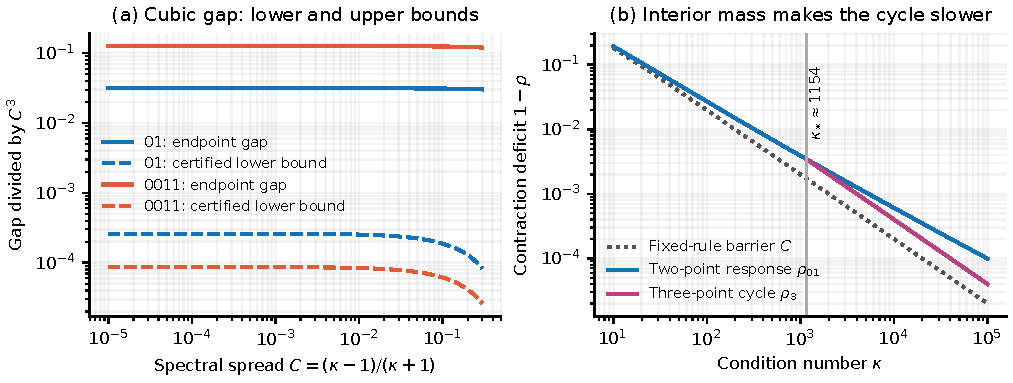
\includegraphics[width=.96\textwidth]{figures/mechanism.pdf}
\caption{Supporting exact-factor mechanisms. Left: the unrestricted gap lies between the conservative transition-frequency certificate and the endpoint gap. These are formula evaluations, not fitted unrestricted factors. Right: above $\kappa_*$ the three-point alternating cycle is slower than the endpoint response.}
\end{figure}

\paragraph{Scope of the numerical illustration.}
The main coefficient figure uses the 113 balanced primitive rotation classes among the 745 exact responses through length 12, together with the 64 recorded equal-block coefficients. Its left panel illustrates the proved density bounds and the two comparison phenomena; its right panel evaluates the exact coefficient formula. The companion \texttt{word\_figure/} directory includes the fixed inputs, generated tables, plotting program, and reproduction instructions. No new optimizer benchmark or empirical fit of $\Gamma$ enters the uniform theorem.

\clearpage
\begin{thebibliography}{99}
\raggedright

\bibitem{AltschulerParrilo2025}
J.~M. Altschuler and P.~A. Parrilo.
Acceleration by stepsize hedging: Silver Stepsize Schedule for smooth convex
optimization.
\emph{Mathematical Programming}, 213:1105--1118, 2025.
\doi{10.1007/s10107-024-02164-2}.

\bibitem{AltschulerParrilo2025a}
J.~M. Altschuler and P.~A. Parrilo.
Acceleration by stepsize hedging: Multi-step descent and the silver
stepsize schedule.
\emph{Journal of the ACM}, 72(2):Article 12, 1--38, 2025.
\doi{10.1145/3708502}.

\bibitem{AzmiKunisch2020}
B.~Azmi and K.~Kunisch.
Analysis of the Barzilai--Borwein step-sizes for problems in Hilbert spaces.
\emph{Journal of Optimization Theory and Applications}, 185(3):819--844, 2020.
\doi{10.1007/s10957-020-01677-y}.

\bibitem{BarzilaiBorwein1988}
J.~Barzilai and J.~M. Borwein.
Two-point step size gradient methods.
\emph{IMA Journal of Numerical Analysis}, 8(1):141--148, 1988.
\doi{10.1093/imanum/8.1.141}.

\bibitem{Billingsley1999}
P.~Billingsley.
\emph{Convergence of Probability Measures}.
Wiley, New York, second edition, 1999.
\doi{10.1002/9780470316962}.

\bibitem{Dai2013}
Y.-H.~Dai.
A new analysis on the Barzilai--Borwein gradient method.
\emph{Journal of the Operations Research Society of China}, 1(2):187--198, 2013.
\doi{10.1007/s40305-013-0007-x}.

\bibitem{DaiFletcherAsymptotic2005}
Y.-H.~Dai and R.~Fletcher.
On the asymptotic behaviour of some new gradient methods.
\emph{Mathematical Programming}, 103:541--559, 2005.
\doi{10.1007/s10107-004-0516-9}.

\bibitem{DaiFletcherProjected2005}
Y.-H.~Dai and R.~Fletcher.
Projected Barzilai--Borwein methods for large-scale box-constrained quadratic programming.
\emph{Numerische Mathematik}, 100:21--47, 2005.
\doi{10.1007/s00211-004-0569-y}.

\bibitem{DaiHagerSchittkowskiZhang2006}
Y.-H.~Dai, W.~W.~Hager, K.~Schittkowski, and H.~Zhang.
The cyclic Barzilai--Borwein method for unconstrained optimization.
\emph{IMA Journal of Numerical Analysis}, 26:604--627, 2006.
\doi{10.1093/imanum/drl006}.

\bibitem{DaiHuangLiu2019}
Y.-H.~Dai, Y.~Huang, and X.-W.~Liu.
A family of spectral gradient methods for optimization.
\emph{Computational Optimization and Applications}, 74:43--65, 2019.
\doi{10.1007/s10589-019-00107-8}.

\bibitem{DaiLiao2002}
Y.-H.~Dai and L.-Z.~Liao.
$R$-linear convergence of the Barzilai and Borwein gradient method.
\emph{IMA Journal of Numerical Analysis}, 22(1):1--10, 2002.
\doi{10.1093/imanum/22.1.1}.

\bibitem{DroriTeboulle2014}
Y.~Drori and M.~Teboulle.
Performance of first-order methods for smooth convex minimization: A novel
approach.
\emph{Mathematical Programming}, 145:451--482, 2014.
\doi{10.1007/s10107-013-0653-0}.

\bibitem{FerrandiHochstenbachKrejic2023}
G.~Ferrandi, M.~E. Hochstenbach, and N.~Kreji\'c.
A harmonic framework for stepsize selection in gradient methods.
\emph{Computational Optimization and Applications}, 85:75--106, 2023.
\doi{10.1007/s10589-023-00455-6}.

\bibitem{FrassoldatiZanniZanghirati2008}
G.~Frassoldati, L.~Zanni, and G.~Zanghirati.
New adaptive stepsize selections in gradient methods.
\emph{Journal of Industrial and Management Optimization}, 4:299--312, 2008.
\doi{10.3934/jimo.2008.4.299}.

\bibitem{GoujaudScieurDieuleveutTaylorPedregosa2022}
B.~Goujaud, D.~Scieur, A.~Dieuleveut, A.~B. Taylor, and F.~Pedregosa.
Super-acceleration with cyclical step-sizes.
In \emph{Proceedings of the 25th International Conference on Artificial
Intelligence and Statistics}, volume 151 of \emph{Proceedings of Machine
Learning Research}, pages 3028--3065, 2022.

\bibitem{Grimmer2024}
B.~Grimmer.
Provably faster gradient descent via long steps.
\emph{SIAM Journal on Optimization}, 34(3):2588--2608, 2024.
\doi{10.1137/23M1588408}.

\bibitem{GrippoSciandrone2002}
L.~Grippo and M.~Sciandrone.
Nonmonotone globalization techniques for the Barzilai--Borwein gradient method.
\emph{Computational Optimization and Applications}, 23:143--169, 2002.
\doi{10.1023/A:1020587701058}.

\bibitem{HuangDaiLiuZhang2020}
Y.~Huang, Y.-H.~Dai, X.-W.~Liu, and H.~Zhang.
Gradient methods exploiting spectral properties.
\emph{Optimization Methods and Software}, 35:681--705, 2020.
\doi{10.1080/10556788.2020.1727476}.

\bibitem{HuangDaiLiu2021}
Y.-K.~Huang, Y.-H.~Dai, and X.-W.~Liu.
Equipping the Barzilai--Borwein method with the two dimensional quadratic
termination property.
\emph{SIAM Journal on Optimization}, 31(4):3068--3096, 2021.
\doi{10.1137/21M1390785}.

\bibitem{HuangDaiLiuZhang2022}
Y.-K.~Huang, Y.-H.~Dai, X.-W.~Liu, and H.~Zhang.
On the asymptotic convergence and acceleration of gradient methods.
\emph{Journal of Scientific Computing}, 90:7, 2022.
\doi{10.1007/s10915-021-01685-8}.

\bibitem{HuangDaiLiuZhang2022b}
Y.-K.~Huang, Y.-H.~Dai, X.-W.~Liu, and H.~Zhang.
On the acceleration of the Barzilai--Borwein method.
\emph{Computational Optimization and Applications}, 81:717--740, 2022.
\doi{10.1007/s10589-022-00349-z}.

\bibitem{LiJiangHong2026}
D.~Li, X.~Jiang, and M.~Hong.
Barzilai--Borwein fails superlinear convergence on an open set of quadratics
for every dimension $n\ge4$.
arXiv:2607.21579, 2026.
\doi{10.48550/arXiv.2607.21579}.

\bibitem{LiSun2021}
D.~Li and R.~Sun.
On a faster $R$-linear convergence rate of the Barzilai--Borwein method.
arXiv:2101.00205, 2021.
\doi{10.48550/arXiv.2101.00205}.

\bibitem{NocedalSartenaerZhu2002}
J.~Nocedal, A.~Sartenaer, and C.~Zhu.
On the behavior of the gradient norm in the steepest descent method.
\emph{Computational Optimization and Applications}, 22(1):5--35, 2002.
\doi{10.1023/A:1014897230089}.

\bibitem{Raydan1993}
M.~Raydan.
On the Barzilai and Borwein choice of steplength for the gradient method.
\emph{IMA Journal of Numerical Analysis}, 13(3):321--326, 1993.
\doi{10.1093/imanum/13.3.321}.

\bibitem{RotaruGlineurPatrinos2026}
T.~Rotaru, F.~Glineur, and P.~Patrinos.
Exact worst-case convergence rates of gradient descent: A complete analysis
for all constant stepsizes over nonconvex and convex functions.
\emph{Mathematical Programming}, 2026.
\doi{10.1007/s10107-025-02313-1}.

\bibitem{SturmanStark2000}
R.~Sturman and J.~Stark.
Semi-uniform ergodic theorems and applications to forced systems.
\emph{Nonlinearity}, 13(1):113--143, 2000.
\doi{10.1088/0951-7715/13/1/306}.

\bibitem{TaylorHendrickxGlineur2017}
A.~B. Taylor, J.~M. Hendrickx, and F.~Glineur.
Exact worst-case performance of first-order methods for composite convex
optimization.
\emph{SIAM Journal on Optimization}, 27(3):1283--1313, 2017.
\doi{10.1137/16M108104X}.

\bibitem{Walters1982}
P.~Walters.
\emph{An Introduction to Ergodic Theory}, volume~79 of \emph{Graduate Texts
in Mathematics}. Springer, New York, 1982.
\doi{10.1007/978-1-4612-5775-2}.

\bibitem{Xu2025}
X.~Xu.
A parameterized Barzilai--Borwein method via interpolated least squares.
\emph{Journal of Industrial and Management Optimization}, 21:6246--6269, 2025.
\doi{10.3934/jimo.2025130}.

\bibitem{YangYuan2026}
S.~Yang and Y.-X.~Yuan.
The sharp worst-case asymptotic rate of the Barzilai--Borwein method in
$\R^d$ and Hilbert spaces.
arXiv:2608.07839, 2026.
\doi{10.48550/arXiv.2608.07839}.

\bibitem{ZhangJiang2026}
Z.~Zhang and R.~Jiang.
Accelerated gradient descent by concatenation of stepsize schedules.
\emph{SIAM Journal on Optimization}, 36(2):1182--1210, 2026.
\doi{10.1137/25M173898X}.

\bibitem{ZhouGaoDai2006}
B.~Zhou, L.~Gao, and Y.-H.~Dai.
Gradient methods with adaptive step-sizes.
\emph{Computational Optimization and Applications}, 35:69--86, 2006.
\doi{10.1007/s10589-006-6446-0}.

\bibitem{YangYuanLyapunov2026}
S.~Yang and Y.-X.~Yuan.
Lyapunov functions and $R$-linear convergence for quadratic
Barzilai--Borwein dynamics.
arXiv:2609.12084, 2026.
\url{https://arxiv.org/abs/2609.12084}.

\bibitem{YangYuanCone2026}
S.~Yang and Y.-X.~Yuan.
$R$-linear convergence of Barzilai--Borwein methods on strictly convex
quadratics via closed-cone homogeneous dynamics.
arXiv:2609.12100, 2026.
\url{https://arxiv.org/abs/2609.12100}.

\bibitem{YangYuanLMSD2026}
S.~Yang and Y.-X.~Yuan.
Global and unconditional $R$-linear convergence of rank-compressed
weighted LMSD sweeps for strictly convex quadratics.
arXiv:2609.12114, 2026.
\url{https://arxiv.org/abs/2609.12114}.


\end{thebibliography}
\end{document}
